\documentclass[american]{ntnuthesis}
% Add support for UTF-8 character set for those engines that do not support it natively.
\usepackage[utf8]{inputenc}

% Handle multi-glyph characters in the output PDF correctly
\usepackage[T1]{fontenc}

% Main font with math support
\usepackage[charter]{mathdesign}
% Sans serif font
\usepackage[scaled=.88]{berasans}
% Monospace font (for code)
\usepackage[scaled=.82]{DejaVuSansMono}

% Verbatim source code environment (code listing)
\usepackage{listings}
% Formatting of code listings
\lstset{%
    frame=single,
    basicstyle=\fontsize{9}{10}\ttfamily,
    keywordstyle=\color{thesisblue}\bfseries,
    stringstyle=\color{thesisred},
    commentstyle=\color{thesisgreen},
    identifierstyle=\color{black},
    numberstyle=\fontsize{7}{8}\selectfont
}

% Consistent language in different packages, such as double quotes with \enquote and
% American-style hyphenation.
\usepackage[american]{babel}

% Page layout
\usepackage{geometry}                   
% Page geometry and spacing (same for even and odd pages)
\geometry{left=4cm, right=4cm, top=4cm, bottom=4.5cm}

% Custom list formatting, such as noitemsep and label
\usepackage{enumitem}
% Itemize and enumerate: tighter and with other symbols
\setlist[enumerate]{itemsep=0mm, topsep=5pt, partopsep=0mm, parsep=0mm}
\setlist[enumerate,1]{label=\arabic*., ref=\arabic*}
\setlist[enumerate,2]{label=\alph*., ref=\alph*}
\setlist[enumerate,3]{label=\roman*., ref=\roman*}
\setlist[itemize]{itemsep=0mm, topsep=5pt, partopsep=0mm, parsep=0mm}
\setlist[itemize,1]{label=$\bullet$}
\setlist[itemize,2]{label=$\circ$}
\setlist[itemize,3]{label=$-$}

% For inserting images into figures
\usepackage{graphicx}                   % including figures
\graphicspath{{./img/}{./tikz/}}

% Common math environments such as \begin{align}, and much, much more.
% Docs: http://texdoc.net/texmf-dist/doc/latex/amsmath/amsldoc.pdf
\usepackage{amsmath}

% Allows definition of colors using \definecolor{}{}{}
\usepackage{xcolor}

% Sub-figures with captions within figures and customisation of captions
\definecolor{dark-gray}{gray}{0.25}
\usepackage[
    font={small,color=dark-gray},
    labelfont={bf, color=black},
    margin=\parindent
]{caption}                    
% Sub-figures with captions within figures
\usepackage[
    font=small,
    labelfont=bf,
    margin=\parindent
]{subcaption}

% Empty pages should be blank
\usepackage{emptypage}

% Recommended for BibLaTeX
% Correctly formatted quotation marks with \enquote{text}
\usepackage{csquotes}                   

% Sitation management.
% Docs: http://ctan.uib.no/macros/latex/contrib/biblatex/doc/biblatex.pdf
% Tutorial: https://www.overleaf.com/learn/latex/Articles/Getting_started_with_BibLaTeX
\usepackage[
    backend=biber,
    style=ieee,
    maxbibnames=99,
    minbibnames=3,
    maxcitenames=2,
    mincitenames=1,
    citestyle=numeric-comp,
    sorting=none,
    dashed=false
]{biblatex}
% Make \fullcite show all authors irrespectively of maxcitenames
\preto\fullcite{\AtNextCite{\defcounter{maxnames}{99}}}

% Tables from csv files
\usepackage{csvsimple}

% Nicer formatting of tables with \toprule, \midrule, and \bottomrule
\usepackage{booktabs}

% Auto-generated filler text
\usepackage{lipsum}

% Used by our custom "algorithm" environment
\usepackage{framed}

% Create figures with semantic code
\usepackage{tikz}
% Allow three-dimensional coordinate specifications
% https://ctan.uib.no/graphics/pgf/contrib/tikz-3dplot/tikz-3dplot_documentation.pdf
% Example usage: https://tex.stackexchange.com/a/212612
\usepackage{tikz-3dplot}
% Allow calculations within curly brackets in tikz figures
\usetikzlibrary{calc, math}
% Adds the braces decoration for showing distances in tikz figures
\usetikzlibrary{decorations.pathreplacing}
% For drawing matrices, useful for masking demonstration
\usetikzlibrary{matrix}
% For bent arrows, amongst others
\usetikzlibrary{arrows}
% Use relative positioning in nodes and paths
% Syntax: below=<optional length> of ...
% https://tex.stackexchange.com/a/25685
\usetikzlibrary{positioning}
% Include .tikz images with \includegraphics, supporting proper scaling
% https://ctan.uib.no/graphics/pgf/contrib/tikzscale/tikzscale.pdf
\usepackage{tikzscale}
% Allow the use of the \spy command in tikz, creating a looking glass effect
% Section 50: http://www.texample.net/media/pgf/builds/pgfmanualCVS2012-11-04.pdf
\usetikzlibrary{spy}

% Proper formatting of units by using \SI{value}{\unit}
% We enable use of \giga\byte and other binary units
\usepackage[binary-units=true]{siunitx}
\DeclareSIUnit\pixel{px}
\DeclareSIUnit\flops{FLOPS}
\sisetup{range-phrase=~--~}

% Wrap text around figures
\usepackage{wrapfig}

% Defines the \vcentcolon symbol, used by the \defeq command
\usepackage{mathtools}

% Allows for H placement specifier in figure environments
% NB! Should be used sparingly.
\usepackage{float}

% Wrapfigure environment for wrapping text around figures
\usepackage{wrapfig}

% Nice inline fractions
\usepackage{nicefrac}

% NB! Should be the last packages defined
% Interactive cross references
\usepackage{hyperref}
% Settings for hyperref: setting all the links black for best printing. They will still be clickable in the PDF
\hypersetup{%
    colorlinks=true,     
    linkcolor=black,    % internal links (change box color with linkbordercolor)
    citecolor=black,    % links to bibliography
    filecolor=black,    % file links
    urlcolor=black      % external links
}

% Automatic cross references
\usepackage[
    capitalize,
    noabbrev
]{cleveref}

% No double spacing between sentences
\frenchspacing

\renewcommand{\lstlistingname}{Code listing}
\renewcommand{\lstlistlistingname}{Code Listings}
\crefname{listing}{Code listing}{Code listings}

\addto\captionsamerican{
\renewcommand{\contentsname}{Contents}
\renewcommand{\listfigurename}{Figures}
\renewcommand{\listtablename}{Tables}
}

% Used for coloring cadastrals
\definecolor{cadastralcolor}{rgb}{0,0,1}

% Colors used for confusions
\definecolor{tp}{HTML}{001F3F}
\definecolor{tn}{HTML}{DDDDDD}
\definecolor{fp}{HTML}{2ECC40}
\definecolor{fn}{HTML}{FF4136}

% Dark green color
\definecolor{darkgreen}{rgb}{0.0, 0.5, 0}

% Colour palette
\definecolor{thesisblue}{rgb}{0.15, 0.15, 0.6}
\definecolor{thesisred}{rgb}{0.4, 0.05, 0.15}
\definecolor{thesisgreen}{rgb}{0.2, 0.3, 0.2}

% Colors used by titled-frame environment employed by algorithm environment
\colorlet{TFFrameColor}{thesisgreen}
\colorlet{TFTitleColor}{white}

% Numeric constants that should stay consistent across entire thesis
\newcommand{\numtiles}{\num{64146}}
\newcommand{\numtesttiles}{\num{9537}}
\newcommand{\numtraintiles}{\num{44939}}
\newcommand{\numvalidationtiles}{\num{9670}}
\newcommand{\numsurfaces}{\num{293336}}

\newcommand{\NTNU}{{N}orwegian {U}niversity of {S}cience and {T}echnology}
\newcommand{\NTNUTrondheim}{{NTNU} in {T}rondheim}

% Vector notation as bold italic symbols
\renewcommand{\vec}[1]{\boldsymbol{#1}}

% Assign value to variable, mostly used in algorithm environment
\newcommand{\assign}[0]{\leftarrow}

% Requires amsmath package
\DeclareMathOperator*{\argmin}{\arg\!\min}
\DeclareMathOperator*{\argmax}{\arg\!\max}

% Defined as equal to, ":="
\newcommand{\defeq}{\vcentcolon=}

% The decomposition of a three-dimensional polygon to two dimensions
\newcommand{\project}[1]{\pi_{\mathrm{2D}}\left(#1\right)}
% The decomposition of a three-dimensional polygon to its planar equation
\newcommand{\planar}[1]{\vec{\beta}\left(#1\right)}
% The (lossy) decomposition of a three-dimensional polygon to its normal vector
\newcommand{\normalplanar}[1]{\vec{n}\left(\planar{#1}\right)}
% Ordinary least squares predictior for the planar equation
\newcommand{\planarestimator}[1]{\widehat{\vec{\beta}}\left(#1\right)}

% Mapping from pixel coordinate to real geographic coordinate
\newcommand{\pixtogeo}[2]{\pi_{B}\left(#1,~#2\right)}

% Big-O notation
\newcommand{\bigo}[1]{\mathcal{O}\left(#1\right)}

% Double bar norm
\newcommand{\norm}[1]{\left\lVert#1\right\rVert}

% Provide relative coordinate in tikz node
\newcommand{\relcoord}[3]{($(#1.south west)!#3!(#1.north west) + (#1.south west)!#2!(#1.south east) - (#1.south west)$)}

% Different types of models, rasters, and so on
\newcommand{\segmodel}[0]{\widehat{f}_{\mathrm{seg}}}
\newcommand{\segmodelparam}[0]{\vec{\theta}_{\mathrm{seg}}}
\newcommand{\normmodel}[0]{\widehat{f}_{\mathrm{norm}}}
\newcommand{\normmodelparam}[0]{\vec{\theta}_{\mathrm{norm}}}
\newcommand{\multitaskmodel}[0]{\widehat{f}_{\mathrm{A,B}}}
\newcommand{\multitaskmodelparam}[0]{\vec{\theta}_{\mathrm{A,B}}}
\newcommand{\singletaskmodelA}[0]{\widehat{f}_{\mathrm{A}}}
\newcommand{\singletaskmodelAparam}[0]{\vec{\theta}_{\mathrm{A}}}
\newcommand{\singletaskmodelB}[0]{\widehat{f}_{\mathrm{B}}}
\newcommand{\singletaskmodelBparam}[0]{\vec{\theta}_{\mathrm{B}}}
\newcommand{\segraster}[0]{S}
\newcommand{\predsegraster}[0]{\widehat{S}}
\newcommand{\predbinarysegraster}[0]{\widetilde{S}}
\newcommand{\normraster}[0]{N}
\newcommand{\predsegnormraster}[0]{\widetilde{N}}
\newcommand{\prednormraster}[0]{\widehat{N}}
\newcommand{\rgbraster}[0]{I}
\newcommand{\lidarraster}[0]{E}
\newcommand{\inputraster}[0]{X}
\newcommand{\polygons}[0]{\mathcal{P}}
\newcommand{\predpolygons}[0]{\widehat{\mathcal{P}}}
\newcommand{\predpolygon}[0]{\widehat{P}}
\newcommand{\simplifiedpolygons}[0]{\widetilde{\mathcal{P}}}
\newcommand{\pseudoinverse}[0]{m^{\dagger}}
\newcommand{\rasterdomain}[0]{R}
\newcommand{\vectordomain}[0]{V}
\newcommand{\predinstraster}[0]{\widehat{L}}

% The first argument becomes the short caption, while the second argument appended to the first becomes the long one
\newcommand{\appcaption}[2]{\caption[#1]{#1 #2}}

% Ceiling and floor operators
\newcommand{\ceil}[1]{\left\lceil #1 \right\rceil}
\newcommand{\floor}[1]{\left\lfloor #1 \right\rfloor}

% Expected value
\newcommand{\E}[1]{\mathrm{E} \left[#1 \right]}
% Variance
\newcommand{\Var}[1]{\mathrm{Var} \left(#1 \right)}
% ReLU activation function
\newcommand{\relu}{\mathrm{ReLU}}
% Approximately proportional to
\newcommand{\appropto}{\mathrel{\vcenter{\offinterlineskip\halign{\hfil$##$\cr\propto\cr\noalign{\kern2pt}\sim\cr\noalign{\kern-2pt}}}}}
% Copyright symbol
\renewcommand{\copyright}[1]{\textcopyright~#1}

% Defines the \normalresult command
\newcommand{\normalresult}[3]{
\begin{tikzpicture}[
  node distance=-0.5em,
]
\def\scaler{0.5}
  \node[](lidar) at (0, 0) {\includegraphics[scale=\scaler]{tile-data/#2-#3/lidar.pdf}};
  \node[below=of lidar](rgb) {\includegraphics[scale=\scaler]{tile-data/#2-#3/rgb.pdf}};
  \node[right=of lidar](predictednormals) {\includegraphics[scale=\scaler]{tile-data/#2-#3/#1/predicted_normals.pdf}};
  \node[below=of predictednormals](truesegmentedpredictednormals) {\includegraphics[scale=\scaler]{tile-data/#2-#3/#1/true_segmented_predicted_normals.pdf}};
  \node[right=of predictednormals](truenormals) {\includegraphics[scale=\scaler]{tile-data/#2-#3/true_normals.pdf}};
  \node[below=of truenormals, xshift=1.3em, yshift=0.155em](cosine) {\includegraphics[scale=0.52]{tile-data/#2-#3/#1/cosine_similarity.pdf}};

  \node[above=-0.25em of lidar.north] {$\lidarraster$};
  \node[above=-0.25em of predictednormals.north] {$\prednormraster$};
  \node[above=-0.25em of truenormals.north] {$\normraster$};
  \node[below=-0.25em of rgb.south] {$\rgbraster$};
  \node[below=-0.25em of truesegmentedpredictednormals.south] {$\segraster \odot \prednormraster$};
  \node[below=-0.25em of cosine.south] {$\mathcal{L}$};
\end{tikzpicture}
}


% Custom algorithm environment
\newcounter{algorithm}
\renewcommand*{\thealgorithm}{Algorithm \arabic{algorithm}}
\newcommand*{\systemautorefname}{algorithm}
\newenvironment{algorithm}[3]
{%
  \refstepcounter{algorithm}\label{#2}
  \begin{titled-frame}{\textbf{\thealgorithm:~}\texttt{#1}}\noindent
  \textbf{Input:}\hspace{1em}\begin{minipage}{\dimexpr\textwidth-3cm}#3\end{minipage}.
  \begin{enumerate}[label=\textbf{\arabic*},leftmargin=0.5cm]%
}
{%
  \end{enumerate}\end{titled-frame}\vspace{0.5em}%
}

% Reference custom algorithm environment
\newcommand{\algref}[1]{\ref{#1}}

% Quick and dirty pseudocode which does not deserve the algorithm environment
\newenvironment{pseudocode}[0]
{%
  \begin{leftbar}
  \noindent
  \hspace{-0.6em}
}
{%
  \end{leftbar}
  \noindent
  \hspace{-0.8em}
}
\newenvironment{pseudoloop}[0]
{%
  \begin{itemize}[nosep,label=,leftmargin=1em]
}
{%
  \end{itemize}
}
\newenvironment{pseudofunc}[2]
{%
  \begin{pseudocode}
  def \textbf{\texttt{#1}}(#2):
  \begin{pseudoloop}
}
{%
  \end{pseudoloop}
  \end{pseudocode}
}


% Title used on front page
\title{Roof Geometry Inference Using Remote Sensing Data}

% Title used in header
\shorttitle{Roof Geometry Inference using Remote Sensing Data}

% Author used on front page
\author{Jakob Gerhard Martinussen}

% Author used in header
\shortauthor{Martinussen}

% Date for front page
\date{\today}

\addbibresource{bib/thesis.bib}
\addbibresource{bib/introduction.bib}
\addbibresource{bib/data.bib}
\addbibresource{bib/cnn.bib}
\addbibresource{bib/segmentation.bib}
\addbibresource{bib/surface-raster.bib}
\addbibresource{bib/optimization.bib}
\addbibresource{bib/post-processing.bib}

\begin{document}

% Metadata content at beginning of content should use roman numbering.
% First abstract should begin on page 3 no matter what, even when the 
% title page is not included
\pagenumbering{roman}
\setcounter{page}{3}

% TODO: Remove before final delivery
\begin{titlepage}
  \maketitle
\end{titlepage}

\chapter*{Abstract}

In this master's thesis, we present an end-to-end machine learning pipeline for inferring the location, orientation, and elevation of flat roof surfaces from remote sensing data (digital surface models and/or aerial photography).
We show that by making a minor modification to the output layer of the U-Net CNN architecture it is able to predict rasterized surface normal vectors with great accuracy.
By clustering predicted normal vectors, using DBSCAN and $k$-NN, it is possible to partition semantic roof segmentation maps into corresponding roof surface instance segmentation maps.
A single multitask CNN architecture which predicts both semantic segmentation masks and rasterized normal vectors is shown to be as performant as a pair of respective single-task networks.
Finally, an optional vectorization procedure which produces three-dimensional vector polygons from roof surface instance segmentation maps is presented.

\chapter*{Sammendrag}

I denne masteroppgaven presenterer vi en ende-til-ende maskinlæringsprosedyre for å identifisere beliggenheten, orientering og høyden til takoverflater ved hjelp av fjernmålinger (digitale overflatemodeller og/eller flyfoto).
Vi viser at ved å gjøre små endringer på utputtlaget til U-Net CNN-arkitekturen evner den å predikere rastrerte overflatenormalvektorer med stor nøyaktighet.
Ved å anvende klyngeanalyse i form av DBSCAN og $k$-NN på de predikerte normalvektorene, så er det mulig å partisjonere semantiske taksegmenteringer til å bli tilsvarende forekomstsegmenteringer hvor hver forekomst representerer en individuell takflate.
Et CNN-nettverk som predikerer både semantiske segmenteringer samt rastrerte normalvektorer har blitt vist til å være like virkningsfull som et par med respektive nettverk som utfører disse to oppgavene uavhengig av hverandre.
En valgfri vektoriseringsprosedyre som produserer tredimensjonale vektorpolygoner fra forekomstsegmenteringer er avslutningsvis presentert.


\cleardoublepage
\tableofcontents
\cleardoublepage
\listoffigures
\cleardoublepage
\listoftables
\cleardoublepage
\listoflistings

\chapter{Introduction}%
\label{sec:introduction}
\pagenumbering{arabic}

\textit{Remote sensing} is the process of gathering information about an object without making physical contact, one such technology being \textit{aerial photography}.
Although aerial RGB photography is intuitively interpretable for humans, it is fundamentally two-dimensional.
\textit{LiDAR}, another remote sensing technology, is able to measure distances to object surfaces by directing a beam of light and measuring the time of arrival and wavelength of the ensuing reflection.
The resulting data can therefore be used to construct a three-dimensional spatial representation of the object of interest.
LiDAR has been applied in a wide array of fields such as meteorology~\cite{lidar_meteorology_1966}, forestry analysis~\cite{lidar_forestry_2000}, urban flood modelling~\cite{lidar_flood_2013}, and autonomous driving systems~\cite{lidar_self_driving_2018}.

One of the applications of LiDAR technology is the construction of \textit{digital surface models} (DSMs).
DSMs are grayscale images representing the earth's surface including all above-surface objects such as natural canopy and human-made objects.
In contrast, \textit{digital terrain models} (DTMs) represent the elevation of the \textit{bare} ground where all above-surface objects have been artificially removed.
While DTMs are often used in geographic and cartographic applications, DSMs can be used for localization and classification of objects above ground.

LiDAR data and aerial photography is usually provided by the respective cadastral authority in a given country.
Cadastral authorities are also responsible for keeping records of cadastral data such as cadastral plots, roads, and buildings.
The exact type and quality of this data varies substantially between countries and sometimes even between administrative regions in the same country.
This raises the question: \enquote{Can high-fidelity insights be inferred from otherwise low-fidelity geographic data?}.
\Cref{fig:data-enchancement} shows an outline of the possible \enquote{data enhancements} which are of interest within this domain. %chktex 2

\begin{figure}
  \includegraphics[width=\linewidth]{data-enchancement}
  \appcaption{%
    Classification of geographic data quality.
  }{%
    The classifications reflect a general observed trend in data sets, and a given region may therefore not fit into exactly one of these categories.
    Some of the data types mentioned here will be described in \cref{sec:data}.
  }%
  \label{fig:data-enchancement}
\end{figure}

The \textit{Norwegian Mapping and Cadastre Authority} (\textit{Statens Kartverk}) provides geographic data of uniquely high quality for the entirety of Norway.
This offers an opportunity to train supervised machine learning models on lower fidelity data in order to infer higher fidelity features.
Such models can then be applied in other regions where only low-fidelity data is available as a method of data enhancement.

The goal of my specialization project~\cite{specialization-project} from \citedate{specialization-project} was to infer two-\linebreak{}dimensional \textit{building outlines} from aerial photography and LiDAR elevation measurements.
A \textit{building outline} is a two-dimensional representation of building \enquote{footprint}.
Such data can be used for map annotations, flood risk analysis, and population density estimates, amongst other applications.
The identification of building outlines from remote sensing data is considered to be medium-fidelity target inference by using low-fidelity features, and can be formulated as a so-called \textit{semantic segmentation} task\footnote{The concepts \enquote{semantic segmentation} and \enquote{instance segmentation} will be formally defined in \cref{sec:segmentation-description}.}.

This master's thesis concerns itself with the reconstruction of three-dimensional \textit{roof surface polygons} from remote sensing data.
Roof surface polygons are completely flat geometries, which when combined form the spatial shape of entire roof structures.
The detection of roof surface polygons is formulated as an \textit{instance segmentation} problem, a task which produces high-fidelity targets.
Three-dimensional representations of roof structures can for example be used for urban planning purposes.
Another application, which incidentally prompted my interest in this topic, is the use of roof surface geometries to estimate the potential energy production of roof-mounted solar panel installations.

The topic of this master's thesis is a natural extension of much of the work already presented in my specialization project.
A sequential two-step method has been developed in order to detect roof surface polygons,
\begin{enumerate}[noitemsep]
  \item Determine which pixels that contain roof structures (semantic segmentation).
  \item Assign a specific roof surface to each \enquote{roof pixel} (instance segmentation).
\end{enumerate}
The first step is essentially a minor reformulation of the task already solved in my specialization project.
For this reason, much of the theory, general methods, and specific source code from my specialization project has been incorporated into this work.

\subsection*{Research questions}

Geographic data, such as building outlines and roof surfaces, are formatted in an unsuitable way for direct machine learning, and must therefore be purposefully transformed and pre-processed.
The development of a data pipeline for geographic data is the first topic of research in this thesis.
%
\begin{description}
  \item[RQ1] How can geographic data representations be transformed into suitable formats for machine learning?
\end{description}
%
After having developed such a pipeline, the focus will be to develop an instance segmentation model for identifying roof surfaces with \emph{raster} data from this pipeline.
The use of aerial photography and LiDAR data from the Norwegian municipality of Trondheim will be investigated, as well as the combination of these two data sources.
%
\begin{description}
  \item[RQ2] How can aerial photography and/or LiDAR data be used in order to infer accurate roof surface instance segmentation maps?
\end{description}
%
The resulting instance segmentation map, which represents rasterized roof surfaces in two dimensions, should be \emph{vectorized}.
That is, the machine learning model's raster predictions should be converted to three-dimensional vector polygons, a data format which is more usable for the most common applications of roof surface geometries.
%
\begin{description}
  \item[RQ3] How can three-dimensional roof surface \emph{polygons} be produced from predicted instance segmentation \emph{raster} maps.
\end{description}
%
Answering this last research question will require the development of additional post-processing methods.

\subsection*{Thesis disposition}

We will start by providing an introduction to the world of \textit{Geographic Information Systems} (GIS); the field which concerns itself with representing geographic data, in \cref{sec:data}.
We will also describe how to pre-process such geographic data in order to produce rasters which are suitable for training accurate machine learning models.
An overview of the problem domain of image segmentation and the methods currently being applied in the field will be provided in \cref{sec:modeling}, a chapter which will also describe the specific model architectures which consume and produce the data formats described in the previous chapter.
The post-processing required in order to produce vectorized surface polygons from predicted rasters will be described in \cref{chap:post-processing}.
Finally, the training procedure and experimental results will be presented and discussed in \cref{sec:experiments}.

The chapter describing geospatial data structures and how they are pre-\linebreak{}processed (\cref{sec:data}) has been placed \emph{before} the chapter about model architectures and techniques related to image segmentation (\cref{sec:modeling}), since the choice of model architecture is highly dependent on how the ground truth target rasters have been constructed.
In order to provide some additional context before describing the pre-processing of our geospatial datasets, we start by giving a formal overview of the problem domains involved in this thesis.
This upcoming section should strictly belong to \cref{sec:modeling}, but the information is still considered essential in order to understand what motivates the decisions made during the pre-processing of the original raw geospatial data.

\section*{Problem description}%
\label{sec:segmentation-description}
For any given image we can pose three relevant \textit{image recognition} questions~\cite{image_recognition}:
%
\begin{enumerate}[]
  \item \textbf{Identification:} Does the image contain any object of interest?
  \item \textbf{Localization:} Where in the image are the objects situated?
  \item \textbf{Classification:} To which categories do the objects belong to?
\end{enumerate}
%
We will concern ourselves with only one object category (class) at any time, that class being roof surfaces, and will simplify the upcoming theory accordingly with this simplification in mind.
The localization and classification of objects in a given image can be performed at different granularity levels, as shown by the \emph{columns} in \cref{fig:segmentation-types}.
The \emph{rows} of \cref{fig:segmentation-types} show how the specific definition of what exactly constitutes an object influences the problem to be solved, where the top row considers entire building to be single objects, while the bottom row considers each individual roof surface to be distinct objects.
It is the latter definition which is of interest in this work.

\begin{figure}[t]
  \includegraphics[width=\linewidth]{segmentation-types}
  \includegraphics[width=\linewidth]{surface-segmentation-types}
  \appcaption{%
    Different granularities for single-class construction localization, using the Trondheim 2017 data set.
  }{%
    Bounding box regression is shown on the left, semantic segmentation in the middle, and instance segmentation on the right.
    The top row defines entire buildings as the objects of interest, while the bottom row considers each individual roof surface as distinct objects.
  }%
  \label{fig:segmentation-types}
\end{figure}

\textit{Bounding box regression} concerns itself with finding the smallest possible rectangles which envelopes the objects of interest.
The sides of the rectangles may either by oriented parallel to the axis directions, or rotated in order to attain the smallest possible envelope.
The bounding box will therefore necessarily contain pixels that are not part of the object itself whenever the object shape is not perfectly rectangular.

\textit{Semantic segmentation} rectifies this issue by classifying each pixel in the image independently, i.e. \textit{pixel-wise} classification, producing a so-called classification \textit{mask}.
\textit{Instance segmentation} distinguishes between pixels belonging to different objects of the same class, while \textit{semantic segmentation} does not make this distinction.
Since a bounding box can be directly derived from a semantic segmentation mask, and a semantic segmentation mask can be directly derived from instance segmentation mask; the problem complexity of these tasks are as follows:
%
\begin{equation*}
  \text{Bounding box regression}
  <
  \text{Semantic segmentation}
  <
  \text{Instance segmentation}.
\end{equation*}
%
An image of width $W$ and height $H$ consisting of $C$ channels is represented by a $W \times H \times C$ tensor, $X \in \mathbb{R}^{W \times H \times C}$.
This is somewhat simplified, but we will give a more nuanced description in \cref{sec:raster-data}.
Single-class semantic segmentation can therefore be formalized as constructing a binary predictor $\tilde{f}$ of the form:
%
\begin{equation*}
  \tilde{f}: \mathbb{R}^{W \times H \times C} \rightarrow \mathbb{B}^{W \times H}, \hspace{2em} \mathbb{B} \defeq \{0, 1\}.
\end{equation*}
%
Where $\mathbb{B}^{W \times H}$ denotes a boolean matrix, $1$ indicating that the pixel is part of the object class of interest, and $0$ indicates the opposite.
In practice, however, statistical models will often predict a pixel-wise class \textit{confidence} in the continuous domain $[0, 1]$,
%
\begin{equation*}
  \hat{f}: \mathbb{R}^{W \times H \times C} \rightarrow {[0, 1]}^{W \times H},
\end{equation*}
%
but a binary predictor can be easily constructed by choosing a suitable threshold, $T$, for which to distinguish positive predictions from negative ones
%
\begin{equation*}
  \tilde{f}(X) = \hat{f}(X) > T, \hspace{2em} X \in \mathbb{R}^{W \times H \times C}.
\end{equation*}
%
The choice of the threshold value $T$ will affect the resulting \textit{sensitivity} and \textit{specificity} metrics of the model predictions, metrics which will be explained in \cref{sec:semantic-segmentation}.

When performing single-class \emph{instance} segmentation, a binary prediction mask is not sufficiently expressive.
Assuming that no more than $m$ individual instances can be simultaneously represented by any given input tensor X, the task is to assign an instance label $l \in \{0, 1, 2, \dots, m\}$ to every single pixel in the input tensor.
The assignment of $l = 0$ means that no object overlaps the given pixel.
An instance predictor $\hat{f}_{\predinstraster}$ is therefore a function producing a label array $\predinstraster$ of the form
\begin{equation*}
  \hat{f}_{\predinstraster}: \mathbb{R}^{W \times H \times C}
  \rightarrow
  \left\{
    0, 1, 2, \dots, m
  \right\}^{W \times H \times C}.
\end{equation*}

Instead of representing each predicted instance as a set of \emph{raster} pixels which share the same label value $l$ in $\predinstraster$, they can be represented as two-dimensional \emph{vectorized} polygons which enclose each given instance instead (\textit{polygon segmentation}).
The specific data format used in order to represent vectorized polygons is presented in \cref{sec:vector-data}.
For the case of three-dimensional objects, the instance polygons can be constructed to be three-dimensional as well, sometimes referred to as \textit{surface segmentation}~\cite{surface-segmentation-1,surface-segmentation-2}.
Since the three-dimensional polygons in a surface segmentation can be projected into a two-dimensional plane in order to produce a polygon segmentation map, and since two-dimensional polygons can be \textit{rasterized} in order to create an instance segmentation map, the problem complexity of these tasks are as follows:
%
\begin{equation*}
  \text{Instance segmentation}
  <
  \text{Polygon segmentation}
  <
  \text{Surface segmentation}.
\end{equation*}

This thesis presents a machine learning pipeline which produces vectorized surface polygon segmentations from remote sensing data.
The pipeline does this by first predicting a semantic segmentation map, which is then partitioned into an instance segmentation map.
This instance segmentation map is then vectorized in order to produce a polygon segmentation map.
Finally, the three dimensional elevation and orientation of each polygon is inferred from the original LiDAR data in order to produce a surface segmentation map.


\chapter{Data and Pre-Processing}%
\label{sec:data}

Geographic data is in wide use by both the public and private sector, and is a huge subject in and of itself.
The storage, processing, and inspection of such data is handled by \textit{Geographic Information Systems} (GIS).
In this section we will explain a few core GIS concepts relevant for the problem at hand, concepts which will inform decisions for how to prepare the data for machine learning purposes.
\Cref{sec:coordinate-systems} will give a brief introduction to the coordinate systems used to represent geographic data.
GIS data can be largely bisected into two categories, vector data and raster data, and both types will be described in \cref{sec:data-types}.
\Cref{sec:data-sets} will present the datasets used for training our models.
The remaining subsections will describe the preprocessing pipeline which has been developed for our specific purposes, preprocessing in the form of cadastral tiling (\cref{sec:tiling-algorithm}), segmentation masking (\cref{sec:masking-algorithm}), and surface rasterization (\cref{sec:surface-rasterization}).
A figurative overview of the preprocessing pipeline is provided by \cref{fig:preprocessing-overview} in \cref{app:preprocessing-overview}.


\section{Coordinate Systems}%
\label{sec:coordinate-systems}
One of the most common coordinate system for representing \textit{arbitrary} positions on earth's surface is the \textit{geographic coordinate system} (GPS).
A given point, $\vec{p} = (\phi, \lambda, z)$, is represented by an angular latitude and longitude, $\phi$ and $\lambda$ respectively, and a radial distance from the mean sea level, $z$.
A negative value for $z$ does not necessarily imply that the given point is below ground, as certain areas (such as in the Netherlands) are situated below sea level.
It is therefore not sufficient to represent elevation data with unsigned floating point numbers.

Although GPS is able to uniquely represent arbitrary geographic points with a high degree of accuracy, it is still unsuitable for many applications.
Cartesian transformations and distance norms are cumbersome to calculate, and data structures and visualizations which are fundamentally two dimensional in nature, such as maps, rasters, and matrices, are difficult to construct from spherical coordinates while protecting important properties of the data.

\begin{wrapfigure}[17]{r}{0.38\linewidth}
  \centering
  \includegraphics[width=0.9\linewidth]{europe-utm-zones.png}
  \caption[UTM zones covering Europe.]{%
    The figure shows the UTM zones required in order to cover the entirety of Europe, from \texttt{29S} to \texttt{38W}.
    This public domain image has been sourced from Wikimedia~\cite{wiki:europe_utm_zones}.
  }%
  \label{fig:europe-utm-zones}
\end{wrapfigure}

In order to solve this problem we define a set of coordinate system \textit{projections} which approximate predefined regions of the earth's surface as flat planes.
The resulting coordinate systems are Cartesian and thus allow us to represent geographic points in the more common $\vec{p} = (x, y, z)$ format.
Cartesian distance norms such as $||\vec{p}_1 - \vec{p}_2||_2$ and Cartesian translations $\vec{p}_1 + \vec{p}_2$ stay within predefined error tolerances as long as operations are contained to the validity region of the given projection.

One such Cartesian approximation of the earth's surface is the Universal Transverse Mercator (UTM) coordinate system which divides the earth into 60 rectangular zones~\cite[p.~48]{map-projections}. The UTM zones covering Europe are shown in \cref{fig:europe-utm-zones}.
We will exclusively use UTM zone \texttt{32V} for our datasets covering the municipality of Trondheim situated in the southern part of Norway.
Data provided in alternative coordinate systems will be mapped to this UTM zone before we start using the data.
Since this is an affine coordinate system, we can easily generalize any models to other coordinate systems by applying the correct affine transformations.
Technical details for how to map between different coordinate systems are given in \cref{app:srid-change} for reproducibility.


\section{Data Types}%
\label{sec:data-types}

We will provide a brief overview of the two main categories of GIS data, namely \textit{vector data} and \textit{raster data}, and how to prepare these data types for machine learning purposes.

\subsection{Vector data}%
\label{sec:vector-data}
A \textit{line string} is an ordered collection of geographic points $(\vec{p}_0, \ldots, \vec{p}_n)$ defining a path which connects each consecutive point by a straight line.
The points are therefore necessarily order dependent.
A \textit{simple} line string is a path which does \textit{not} intersect itself, while a \textit{complex} line string is one that does.
When the first and last points of a line string are identical it is considered a \textit{linear ring}, i.e.\ $l = (\vec{p}_0, \ldots, \vec{p}_n, \vec{p}_0)$.
A \textit{polygon} can therefore be represented by a simple linear ring which defines its \textit{exterior hull} and any number of simple linear strings which defines its \textit{interior hulls}.
\Cref{fig:polygon-representation} illustrates these concepts for polygons with and without interior hulls. % chktex 2

\begin{figure}[H]
  \centering
  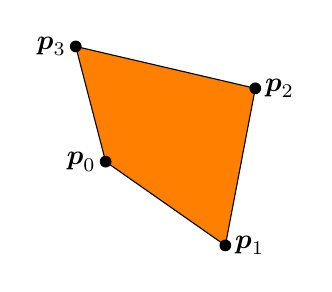
\begin{tikzpicture}[scale=1.9,yscale=0.7]
  \coordinate (zero) at (0, 0);
  \coordinate (one) at (0.8, -0.8);
  \coordinate (two) at (1, 0.7);
  \coordinate (three) at (-0.2, 1.1);
  \draw[fill=orange]
    (zero) node[left] {$\vec{p}_0$}
    -- (one) node[right] {$\vec{p}_1$}
    -- (two) node[right] {$\vec{p}_2$}
    -- (three) node[left] {$\vec{p}_3$}
    -- cycle;
  \foreach \n in {zero,one,two,three}
    \node at (\n)[circle,fill,inner sep=1.5pt]{};
\end{tikzpicture}

  \textcolor{gray}{\vrule}
  \hspace{0.01\linewidth}
  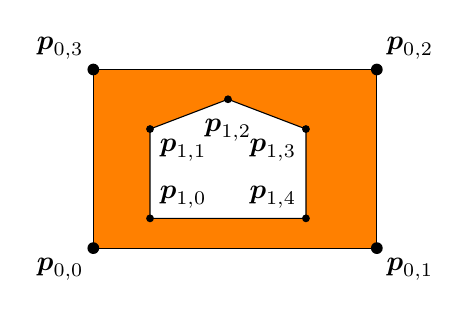
\begin{tikzpicture}[scale=1.8,yscale=0.7]
  \coordinate (zero) at (0, 0);
  \coordinate (one) at (2.0, 0);
  \coordinate (two) at (2.0, 1.8);
  \coordinate (three) at (0, 1.8);
  \draw[fill=orange]
    (zero) node[below left] {$\vec{p}_{0,0}$}
    -- (one) node[below right] {$\vec{p}_{0,1}$}
    -- (two) node[above right] {$\vec{p}_{0,2}$}
    -- (three) node[above left] {$\vec{p}_{0,3}$}
    -- cycle;
  \foreach \n in {zero,one,two,three}
    \node at (\n)[circle,fill,inner sep=1.5pt]{};

  \coordinate (0) at (0.4, 0.3);
  \coordinate (1) at (1.5, 0.3);
  \coordinate (2) at (1.5, 1.2);
  \coordinate (3) at (0.95, 1.5);
  \coordinate (4) at (0.4, 1.2);
  \draw[fill=white]
    (0) node[above right] {$\vec{p}_{1,0}$}
    -- (1) node[above left] {$\vec{p}_{1,4}$}
    -- (2) node[below left] {$\vec{p}_{1,3}$}
    -- (3) node[below=3.5pt] {$\vec{p}_{1,2}$}
    -- (4) node[below right] {$\vec{p}_{1,1}$}
    -- cycle;
  \foreach \n in {0,1,2,3,4}
    \node at (\n)[circle,fill,inner sep=1pt]{};
\end{tikzpicture}

  \caption[Types of vectorized polygons.]{%
    Simple polygon with four unique vertices is shown on the left hand side.
    A complex polygon with an outer hull
    and an interior hull is shown on the right hand side for comparison.
  }%
  \label{fig:polygon-representation}
\end{figure}

A polygon is considered invalid if one or more of its linear rings are self-intersecting, i.e.\ if any of its rings is considered to be complex.
Data providers frequently provide polygons in invalid states and such polygons must be corrected since they are often not processable by common GIS tools.
Zero-buffering invalid polygons (growing the polygon in all directions by zero units) fixes such problems, as can be seen in \cref{fig:complex-zero-buffer}.

\begin{figure}[H]
  \centering
  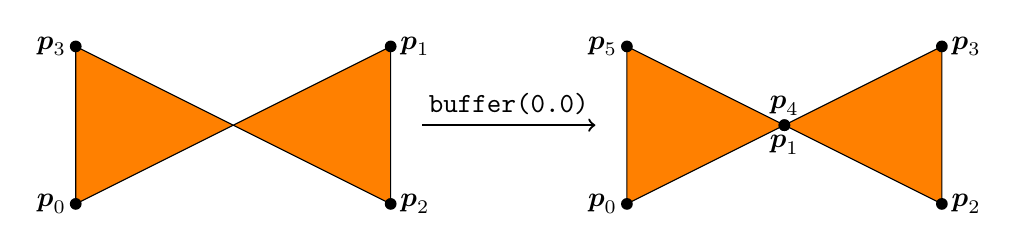
\begin{tikzpicture}[scale=1]
  \coordinate (ll) at (0, 0);
  \coordinate (mid) at (2, 1);
  \coordinate (lr) at (4, 0);
  \coordinate (ur) at (4, 2);
  \coordinate (ul) at (0, 2);
  \draw[fill=orange]
    (ll) node[left] {$\vec{p}_0$}
    -- (ur) node[right] {$\vec{p}_1$}
    -- (lr) node[right] {$\vec{p}_2$}
    -- (ul) node[left] {$\vec{p}_3$}
    -- cycle;
  \foreach \n in {ll,ur,lr,ul}
    \node at (\n)[circle,fill,inner sep=1.5pt]{};

   \draw (4.4, 1) edge[->, thick] node[above] {\texttt{buffer(0.0)}} (6.6, 1);

  \coordinate (offset) at (7, 0);
  \draw[fill=orange]
    ($ (ll) + (offset) $) node[left] {$\vec{p}_0$}
    -- ($ (mid) + (offset) $) node[below] {$\vec{p}_1$}
    -- ($ (lr) + (offset) $) node[right] {$\vec{p}_2$}
    -- ($ (ur) + (offset) $) node[right] {$\vec{p}_3$}
    -- ($ (mid) + (offset) $) node[above] {$\vec{p}_4$}
    -- ($ (ul) + (offset) $) node[left] {$\vec{p}_5$}
    -- cycle;
  \foreach \n in {ll,mid,lr,ur,mid,ul}
    \node at ($ (\n) + (offset) $)[circle,fill,inner sep=1.5pt]{};
\end{tikzpicture}

  \caption{Illustration of how zero-buffering an invalid polygon corrects self-intersecting polygons.}%
  \label{fig:complex-zero-buffer}
\end{figure}

Zero-buffering polygons has the added benefit of normalizing vector data by re-ordering the polygon vertices in an anti-clockwise manner and removing redundant vertices as shown in \cref{fig:redundant-zero-buffer}.

\begin{figure}[H]
  \centering
  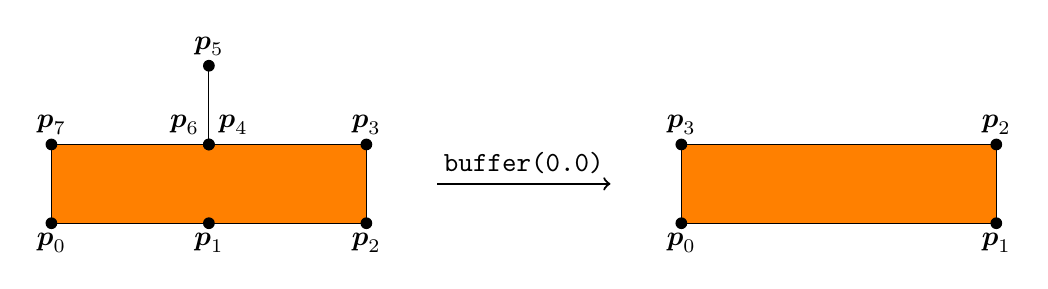
\begin{tikzpicture}[scale=1]
  \coordinate (ll) at (0, 0);
  \coordinate (lm) at (2, 0);
  \coordinate (lr) at (4, 0);
  \coordinate (ur) at (4, 1);
  \coordinate (um) at (2, 1);
  \coordinate (Um) at (2, 2);
  \coordinate (ul) at (0, 1);
  \draw[fill=orange]
    (ll) node[below] {$\vec{p}_0$}
    -- (lm) node[below] {$\vec{p}_1$}
    -- (lr) node[below] {$\vec{p}_2$}
    -- (ur) node[above] {$\vec{p}_3$}
    -- (um) node[above right] {$\vec{p}_4$}
    -- (Um) node[above] {$\vec{p}_5$}
    -- (um) node[above left] {$\vec{p}_6$}
    -- (ul) node[above] {$\vec{p}_7$}
    -- cycle;
  \foreach \n in {ll,lm,lr,ur,um,Um,um,ul}
    \node at (\n)[circle,fill,inner sep=1.5pt]{};

   \draw (4.9, 0.5) edge[->, thick] node[above] {\texttt{buffer(0.0)}} (7.1, 0.5);

  \coordinate (offset) at (8, 0);
  \draw[fill=orange]
    ($ (ll) + (offset) $) node[below] {$\vec{p}_0$}
    -- ($ (lr) + (offset) $) node[below] {$\vec{p}_1$}
    -- ($ (ur) + (offset) $) node[above] {$\vec{p}_2$}
    -- ($ (ul) + (offset) $) node[above] {$\vec{p}_3$}
    -- cycle;
  \foreach \n in {ll,lr,ur,ul}
    \node at ($ (\n) + (offset) $)[circle,fill,inner sep=1.5pt]{};
\end{tikzpicture}

  \caption{Illustration of how zero-buffering polygons removes redundant vertices.}%
  \label{fig:redundant-zero-buffer}.
\end{figure}

This allows you to apply simpler similarity measures for comparing polygons, and reduces computational costs when processing the polygons.
Technical details for applying zero-buffers to vector data is provided in \cref{app:zero-buffer}.
We will come back to how to combine vector and raster datasets by \textit{rasterization} in \cref{sec:masking-algorithm} where it will also become clear why the removal of redundant vertices is of importance.


\subsection{Raster data}%
\label{sec:raster-data}
Raster data consists of a set of scalar measurements imposed onto a grid.
A color image, $\rgbraster$, of width $\mathrm{W}$ and height $\mathrm{H}$, will contain three color channels; red, green, and blue (RGB), and can be represented by a three-dimensional array of size $\mathrm{H} \times \mathrm{W} \times \mathrm{3}$.
Each color channel for a given pixel is represented by an unsigned 8-bit integer, i.e.
%
\begin{equation*}
  \rgbraster_{i, j, c} \in \{0, 1, \ldots, 255\},
  \hspace{2.5em}
  i = 1, \ldots, \mathrm{H} ,
  ~~
  j = 1, \ldots, \mathrm{W},
  ~~
  c = \mathrm{\textcolor{red}{r}, \textcolor{green}{g}, \textcolor{blue}{b}}.
\end{equation*}
%
A LiDAR elevation map, which we will denote as $\lidarraster$, is likewise encoded as a single-channel grayscale image of size $\mathrm{W} \times \mathrm{H}$.
Each pixel is represented by a signed 32-bit floating point value which gives the following approximate value domain
%
\begin{equation*}
  \lidarraster_{i, j} \in \mathbb{R},
  \hspace{2.5em}
  i = 0, \ldots, \mathrm{H} - 1,
  ~~
  j = 0, \ldots, \mathrm{W} - 1.
\end{equation*}
%
These two raster types must be handled differently during data-standardization and -normalization due to their different value domains, which we will come back to in \cref{sec:raster-normalization}.
Whenever we refer to remote sensing raster data in \emph{general}, be it LiDAR and/or RGB, we will denote the input raster as $\inputraster$.

For GIS rasters specifically we must additionally provide the spatial extent of the given raster defined by:
\begin{itemize}[noitemsep]
  \item A coordinate system, for example UTM \texttt{32V}.
  \item The coordinate of the center of the upper left pixel, $\inputraster_{1, 1}$; the \textit{origin} $\vec{r}_0 = {[x_0, y_0]}^T$.
  \item The pixel step size, $\vec{\Delta} = {[\Delta_x, \Delta_y]}^T$, for example ${[\SI{0.25}{\meter}, \SI{-0.25}{\meter}]}^T$.
\end{itemize}

The pixel value $\inputraster_{i, j, c}$ therefore represents a rectangle of width $\Delta_x$ and height $\Delta_y$ centered at the spatial coordinate $\vec{r}_0 + [\Delta_y i, \Delta_x j]$ interpreted in the given coordinate system.

Missing data in remote sensing rasters is specified by filling in a predefined \texttt{nodata} placeholder value.
For RGB data this is often set to $0$, resulting in a black pixel.
LiDAR rasters often use $\texttt{nodata} = -2^{127} \times (2 - 2^{-23}) \approx -3.4028234664 \times 10^{38}$, the most negative normal number representable by a single-precision floating point number.
Such \texttt{nodata} values may arise from measurement errors or by pixels situated outside the given coverage area of the dataset, and must be special-cased during data normalization, which we will come back to in \cref{sec:raster-normalization}.

When we will train models on the combination of LiDAR and aerial photography data, these two types of rasters must be merged in order to attain a consistent three-dimensional array of size $H \times W \times 4$.
These rasters can not be simply superposed when their pixel sizes $\vec{\Delta}$ and/or origins $\vec{r}_0$ differ.
In such cases we will apply bilinear interpolation on the raster of greatest resolution and subsequently downsample it in order to align all pixels.
See \cref{app:raster-merging} for how this is performed in practice.


\section{Datasets}%
\label{sec:data-sets}

The modelling results presented in \cref{sec:experiments} are trained on GIS data covering the Norwegian municipality of Trondheim.
All datasets, except from the three-dimensional roof polygon dataset kindly provided by Norkart, have been made available by the \enquote{Norge digitalt}-partnership and have been downloaded from \url{https://geonorge.no}, an online service hosted by \textit{Norwegian Mapping and Cadastre Authority} (\textit{Statens Kartverk}).
All data, unless otherwise stated, are licenced under the \enquote{Norge digitalt}-licence\footnote{Information regarding the \enquote{Norge digitalt}-licence can be found here: \url{https://www.geonorge.no/Geodataarbeid/Norge-digitalt/Avtaler-og-maler/Norge-digitalt-lisens/}.} which restricts the use to non-commercial purposes.

\subsection{Raster datasets}
We will use the \enquote{Ortofoto Trondheim 2017}\footnote{Product specification for \enquote{Ortofoto Trondheim 2017} can be found here:\\ \url{https://kartkatalog.geonorge.no/metadata/cd105955-6507-416f-86d2-6d95c1b74278}.} aerial photography dataset from 2017 which requires \SI{161}{\giga\byte} of storage space.
The real image resolution is \SIrange{0.04}{0.15}{\meter}, but is provided with an resampled resolution of \SI{0.1}{\meter} for consistency, that is, each pixel is of size $\SI{0.1}{\meter} \times \SI{0.1}{\meter}$.
The reported accuracy is \SI{\pm 0.35}{\meter}~\cite{trondheim_ortophoto_2017}, although the exact type of this accuracy is not specified.
An exemplified region is visualized in \cref{fig:rgb-example}.

\begin{figure}[hbt]
  \centering
  \includegraphics[width=0.75\linewidth]{data/rgb-example}
  \appcaption{%
    Visualization of the \enquote{Ortofoto Trondheim 2017} aerial photography dataset.
  }{%
    \copyright{Kartverket}.
  }%
  \label{fig:rgb-example}
\end{figure}

An \textit{orthophoto} is an image where the geographic scale is uniform over the entire image.
Proper orthophotos are expensive to manufacture and are therefore seldomly available for most geographic regions~\cite{ortofoto_in_norway_2003}, including Trondheim.
Aerial photography which has not been properly \enquote{ortho-rectified} may impede location-based inference as there exists no exact one-to-one mapping between image pixels and geographic coordinates.
This problem is best understood by an example, as shown in \cref{fig:non-orthophoto-example}.

\begin{figure}[hbt]
  \centering
  \begin{tikzpicture}
    \node[anchor=south west,inner sep=0] (image) at (0,0) {\includegraphics[width=0.75\linewidth]{data/non-orthophoto-example}};
    \begin{scope}[x={(image.south east)},y={(image.north west)}]
      \draw[orange, ultra thick, fill=orange!50, fill opacity=0.25]
        (0.34, 0.3) --
        (0.615, 0.55) --
        (0.61, 0.69) --
        (0.33, 0.445) --
        cycle;
    \end{scope}
  \end{tikzpicture}
  \appcaption{%
    Example of nonproper orthophoto.
  }{%
    The building centered in the image is 14 stories tall.
    The orange area annotates a clearly visible building wall.
    \copyright{Kartverket}.
  }%
  \label{fig:non-orthophoto-example}
\end{figure}

As can be seen in \cref{fig:non-orthophoto-example}, the \enquote{Ortofoto Trondheim 2017} dataset clearly shows one side of a building due to the perspective of the plane capturing the image.
An ideal orthophoto would capture all vertical building walls as single, straight lines, no matter the perspective.
The effect of this \enquote{parallax error} on semantic segmentation predictions has been investigated in our previous work~\cite{specialization-project}, the conclusion being that it does \emph{not} impede predictive accuracy to a major degree.

The LiDAR dataset used is \enquote{Høydedata Trondheim 5pkt 2017}\footnote{Product specification for \enquote{Høydedata Trondheim 5pkt 2017} can be found here:\\ \url{https://kartkatalog.geonorge.no/metadata/bec4616f-9a62-4ecc-95b0-c0a4c29401dc}.} from \date{2017-10-10} and requires \SI{25}{\giga\byte} of storage space.
The pixel size is $\SI{0.25}{\meter} \times \SI{0.25}{\meter}$ and the LiDAR measurements have a reported standard deviation of \SI{0.02}{\meter}~\cite{trondheim_lidar_2017}.
LiDAR visualized as a grayscale image over the same region as in \cref{fig:rgb-example} is presented in \cref{fig:lidar-example}.

\begin{figure}[hbt]
  \centering
  \includegraphics[width=0.75\linewidth]{data/lidar-example}
  \caption[Visualization of LiDAR data from Trondheim.]{%
    Visualization of the \enquote{Høydedata Trondheim 5pkt 2017} LiDAR dataset.
    \copyright{Kartverket}.
  }%
  \label{fig:lidar-example}
\end{figure}


\clearpage
\subsection{Vector datasets}
The \enquote{Matrikkelen - Eiendomskart Teig}\footnote{Product specification for \enquote{Matrikkelen - Eiendomskart Teig} can be found here:\\\url{https://kartkatalog.geonorge.no/metadata/74340c24-1c8a-4454-b813-bfe498e80f16}.} data set contains all cadastral plots in Trondheim, the use of which will be explained in \cref{sec:tiling-algorithm}.
The \enquote{FKB-bygning}\footnote{Product specification for \enquote{FKB-bygning} can be found here:\\\url{https://kartkatalog.geonorge.no/metadata/8b4304ea-4fb0-479c-a24d-fa225e2c6e97}.} data set contains all registered building outlines in Trondheim.
The building outlines will be used to construct binary classification masks as outlined in \cref{sec:masking-algorithm}.
Both data sets are illustrated in \cref{fig:vector-data-example}.

\begin{figure}[htb]
  \includegraphics[trim={5cm 0 5cm 0},clip, width=0.49\linewidth]{data/teig-example}
  \includegraphics[trim={5cm 0 5cm 0},clip, width=0.49\linewidth]{data/building-example}
  \caption{%
    Illustration of vector data sets.
    Cadastral plots are shown on the left while building outlines are shown on the right.
    \copyright{Kartverket}.
  }%
  \label{fig:vector-data-example}
\end{figure}


\section{Tiling Algorithm}%
\label{sec:tiling-algorithm}
The data sets provided to us are in a state unsuitable for direct use by machine learning frameworks.
For this reason we need to develop a preprocessing pipeline that transforms the data into a more customary format.
The data preprocessing should be generalizable to different regions, data formats, data types (vector vs.\ raster), coordinate systems, and so on.
The goal is to implement a modelling pipeline that can be applied to other geographic regions in the future.

Our data sets are defined over a single, contiguous geographic area, and we must therefore define a \textit{sample space} which allows us to split the data into training-, validation-, and test-sets.
The collection of all cadastral plots in a given region is a suitable sample space since cadastral plots are non-overlapping regions of relatively small size and have a high probability of containing one or more buildings.
A large raster dataset covering a sparsely populated region can therefore be substantially reduced in size before training.
An alternative approach is to split the entire data set into regularly sized tiles and use this tile collection as the sample space.
A tiled sample space, for anything other than densely populated areas, will suffer from class imbalances due to low building densities in most tiles.

Given a specific geographic region, defined by the extent of the cadastral plot, we must retrieve the raster which covers the region of interest.
The simplest approach is to calculate the \textit{axis-aligned bounding box} of the plot, the minimum-area enclosing rectangle of the given plot.
A bounding box is uniquely defined by its centroid $\vec{c} = [\nicefrac{1}{2}(x_{\mathrm{\min}} + x_{\mathrm{\max}}), \nicefrac{1}{2}(y_{\mathrm{\min}} + y_{\mathrm{\max}})]$, width $w = x_{\mathrm{\max}} - x_{\mathrm{\min}}$, and height $h = y_{\mathrm{\max}} - y_{\mathrm{\min}}$, and we will denote it by $B(\vec{c}, w, h)$.
This is shown in \cref{fig:cadastral-bbox}.

\begin{figure}[htb]
  \captionsetup[subfigure]{position=b}
  \centering
  \subcaptionbox{
    Bounding box calculation for a given cadastral.
    The cadastral is shown in \textcolor{orange}{orange},
    and the resulting bounding box is annotated with \textcolor{blue}{blue} dashed lines.%
    \label{fig:cadastral-bbox}
  }{
    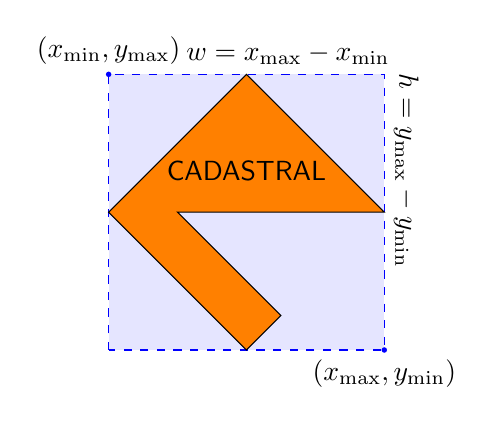
\begin{tikzpicture}[scale=0.035]
  \tikzmath{
    \xmin=0;
    \xmax=100;
    \ymin=0;
    \ymax=100;
    \xmid=0.5 * \xmin + 0.5 * \xmax;
    \ymid=0.5 * \ymin + 0.5 * \ymax;
  }
  \coordinate (lr) at (\xmax, \ymin);
  \coordinate (ul) at (\xmin, \ymax);

  \draw[dashed, color=cadastralcolor, fill=cadastralcolor!10] (\xmin, \ymin) rectangle (\xmax, \ymax);
  \filldraw[orange, draw=black] (50, \ymin) -- (62.5, 12.5) -- (25, 50) -- (\xmax, 50) -- (50, \ymax) -- (0, 50) -- cycle;

  \draw (ul) node[above] {$(x_{\mathrm{min}}, y_{\mathrm{max}})$};
  \fill[cadastralcolor] (ul) circle [radius=1];

  \draw (lr) node[below] {$(x_{\mathrm{max}}, y_{\mathrm{min}})$};
  \fill[cadastralcolor] (lr) circle [radius=1];

  \draw (\xmid, \ymax) node[above] {$\hspace{3em}w = x_{\mathrm{max}} - x_{\mathrm{min}}$};
  \draw (\xmax, \ymid) node[above, rotate=-90] {$\hspace{-3em}h = y_{\mathrm{max}} - y_{\mathrm{min}}$};

  \draw (\xmid, 65) node[scale=1, black] {\textsf{CADASTRAL}};
\end{tikzpicture}

  }
  \hspace{2em}
  \subcaptionbox{
    Figure showing the difference between a regular bounding box shown in
    \textcolor{blue}{blue}, and a minimum rotated rectangle shown in
    \textcolor{red}{red}.
    Angle of rectangle rotation denoted by $\phi$.%
    \label{fig:rotated-bbox}
  }{
    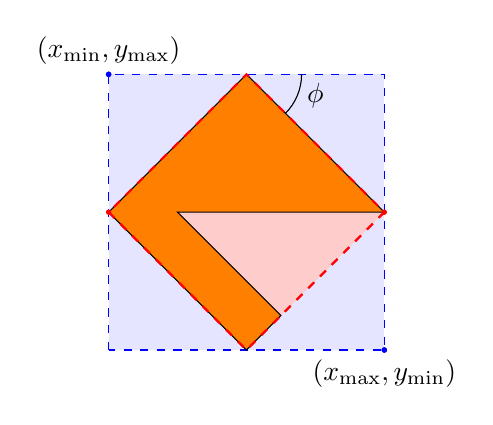
\begin{tikzpicture}[scale=0.035]
  \tikzmath{
    \xmin=0;
    \xmax=100;
    \ymin=0;
    \ymax=100;
    \xmid=0.5 * \xmin + 0.5 * \xmax;
    \ymid=0.5 * \ymin + 0.5 * \ymax;
  }
  \coordinate (lr) at (\xmax, \ymin);
  \coordinate (ul) at (\xmin, \ymax);

  \draw[dashed, color=cadastralcolor, fill=cadastralcolor!10] (\xmin, \ymin) rectangle (\xmax, \ymax);
  \draw[dashed, color=red, fill=red!20, fill opacity=1] (\xmin, 50) -- (50, \ymin) -- (\xmax, 50) -- (50, \ymax) -- cycle; 
  \filldraw[orange, draw=black] (50, \ymin) -- (62.5, 12.5) -- (25, 50) -- (\xmax, 50) -- (50, \ymax) -- (0, 50) -- cycle;
  \draw[dashed, thick, color=red] (\xmin, 50) -- (50, \ymin) -- (\xmax, 50) -- (50, \ymax) -- cycle; 

  \fill[cadastralcolor] (ul) circle [radius=1];
  \fill[cadastralcolor] (lr) circle [radius=1];

  \fill[red] (\xmin, 50) circle [radius=1];
  \fill[red] (\xmax, 50) circle [radius=1];

  % Draw angle of rotation
  \draw[black] (\xmid + 20, \ymax) arc [start angle=0, end angle=-45, radius=20] node[midway, right] {$\phi$};

  % The following is added such that the resulting figure has the same dimensions as cadastre_bbox
  \draw (ul) node[above] {$(x_{\mathrm{min}}, y_{\mathrm{max}})$};
  \fill[cadastralcolor] (ul) circle [radius=1];
  \draw (lr) node[below] {$(x_{\mathrm{max}}, y_{\mathrm{min}})$};
  \fill[cadastralcolor] (lr) circle [radius=1];
\end{tikzpicture}

  }
  \caption{Comparison of bounding box methods.}
\end{figure}

The edges of the bounding box is by definition oriented parallel to the coordinate axes.
An alternative method is to calculate the \textit{arbitrarily oriented minimum bounding box} (AOMBB), a rectangle rotated by $\phi$ degrees w.r.t.\ the $x$-axis, as shown in \cref{fig:rotated-bbox}.

While AOMBB yields regions with less superfluous raster data, it requires warping of the original raw raster whenever $\phi$ is not a multiple of \SI{90}{\degree}, i.e.\ $\phi \not\in \{ \SI{0}{\degree}, \SI{90}{\degree}, \SI{180}{\degree}, \SI{270}{\degree} \}$.
Such warping requires data interpolation of the original raster data due to the rotation of the coordinate system, and may introduce artifacts to the warped raster without careful parameter tuning.
AOMBB is therefore not a viable approach during the preprocessing stage, and we will therefore use axis-aligned minimum bounding boxes instead, from now on simply referred to as \textit{bounding boxes}.

Calculating bounding boxes for the cadastral plots in our data sets will yield rectangles of variable dimensions.
Variable input sizes will cause issues for model architectures which require predefined input dimensions.
Convolutional neural networks do handle variable input sizes, but dimensions off all images in a \textit{single} training batch must be of the same size.
It is therefore preferable to normalize the size of each bounding box.

The distributions of the bounding box widths ($w$), heights ($h$), and maximal dimensions ($m = \max \{w, h\}$) are shown in \cref{fig:bbox-stats}.

\begin{figure}[htb]
  \includegraphics[width=\linewidth]{bbox_stats}
  \caption[Distribution of bounding box dimensions.]{%
    Distribution of bounding box widths $w$ (left), heights $h$ (middle), and largest dimension $m = \max \{w, h\}$ (right).
    The cut-off value of $\SI{64}{\meter}$ is shown by \textcolor{red}{red} dotted vertical lines.
    The fraction of bounding boxes with dimension $\leq \SI{64}{m}$ is annotated as well.
    The $x$-axis has been cut off at the 90th percentile.
    \textit{Dataset: Trondheim cadastre}.
  }%
  \label{fig:bbox-stats}
\end{figure}

As can be seen in \cref{fig:bbox-stats}, the distributions of $h$ and $w$ are quite similar, as expected.
A square $1:1$ aspect ratio is therefore suitable for the normalized bounding box size.
Specifically, a $\SI{64}{\meter} \times \SI{64}{\meter}$ bounding box will be of sufficient size to contain $\approx \SI{85}{\percent}$ of all cadastre plots in a single tile.
With a LiDAR resolution of $\SI{0.25}{\meter}$, this results in a final image resolution of $\SI{256}{\pixel} \times \SI{256}{\pixel}$.
This resolution has the added benefit of being a common resolution for CNNs.

How should the bounding boxes be normalized to to $\SI{256}{\pixel} \times \SI{256}{\pixel}$?
A common technique is to resize the original image by use of methods such as bilinear interpolation or Lanczos resampling.
While this is tolerable for normal photographs, where each pixel has a variable surface area mapping, it is an especially lossy transformation for remote sensing data.
In the Trondheim 2017 LiDAR data set, for instance, each pixel represents a $\SI{0.25}{\meter} \times \SI{0.25}{\meter}$ real world area.
If the highly variable extent of each bounding box is scaled to $\SI{256}{\pixel} \times \SI{256}{\pixel}$, the real world area of each pixel will differ greatly between cadastral plots.
Resized images will also become distorted whenever the original aspect ratio is not $1:1$.

A better method utilizes the fact that the remote sensing data covers a continuous geographic region, which allows us to expand the feature space beyond the original region of interest.
The original bounding box is denoted as $B(\vec{c}, w, h)$.
Now, define the following \enquote{enlarged} width and height:
%
\begin{align*}
  h^* &:= \ceil{\frac{h}{\SI{64}{\meter}}} \cdot \SI{64}{\meter},
  \hspace{3em}
  w^* := \ceil{\frac{w}{\SI{64}{\meter}}} \cdot \SI{64}{\meter}
\end{align*}
%
The new bounding box, $B(\vec{c}, w^*, h^*)$, covers the original bounding box and is divisible by \SI{256}{\pixel} in both dimensions.
In other words, the original bounding box is grown in all directions until both the width and height are multiples of \SI{64}{\meter} (\SI{256}{\pixel}).
This is demonstrated in \cref{fig:bbox-growing}.

\begin{figure}[H]
  \centering
  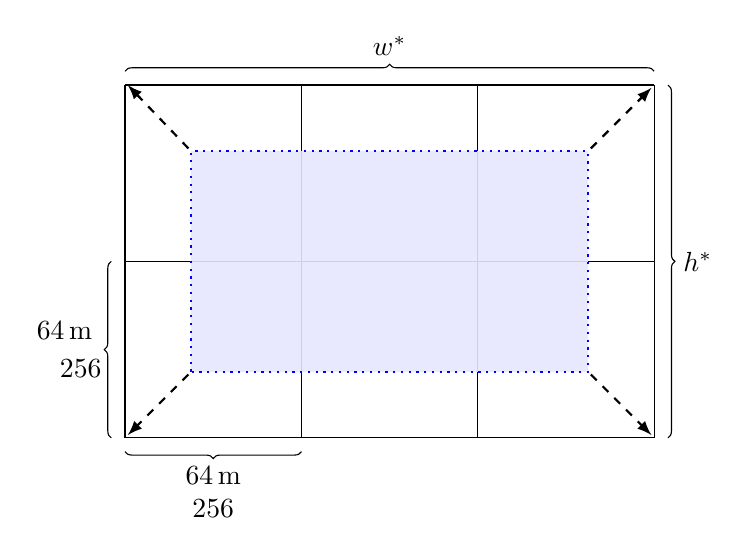
\begin{tikzpicture}[scale=0.035]
  \tikzmath{
    \tile=64;
    \bboxwidth=2.25 * \tile;
    \collectionwidth=3 * \tile;
    \bboxheight=1.25 * \tile;
    \collectionheight=2 * \tile;
    \offset = 0.375 * \tile;
    \shift = 5;
  }
  \draw (0, 0) grid[step=\tile] (\collectionwidth, \collectionheight);

  % Show tile dimensions
  \draw[decoration={brace}, decorate]
    (-\shift, 0) -- node[above left] {$\SI{64}{\metre}~$} node[below left] {$\SI{256}{\pixel}$} (-\shift, \tile);

  \draw[decoration={brace,mirror}, decorate]
    (0, -\shift) -- node[below=2pt, align=center] {$\SI{64}{\metre}$ \\ $\SI{256}{\pixel}$} (\tile, -\shift);

  % Show dimensions of tile collection
  \draw[decoration={brace,mirror}, decorate]
    (\collectionwidth + \shift, 0) 
    --
    node[right=2pt]{$h^*$}
    (\collectionwidth + \shift, \collectionheight);
  \draw[decoration={brace}, decorate]
    (0, \collectionheight + \shift) 
    --
    node[above=2pt]{$w^*$}
    (\collectionwidth, \collectionheight + \shift);

  % Arrows showing growth of bounding box
  \tikzset{>=latex}
  \draw (\bboxwidth + \offset + 1, \offset - 1) edge[->, thick, dashed] (\collectionwidth - 1, 1);
  \draw (\bboxwidth + \offset + 1, \bboxheight + \offset + 1) edge[->, thick, dashed] (\collectionwidth - 1, \collectionheight - 1);
  \draw (\offset - 1, \bboxheight + \offset + 1) edge[->, thick, dashed] (1, \collectionheight);
  \draw (\offset - 1, \offset - 1) edge[->, thick, dashed] (1, 1);

  % Draw original bounding box
  \draw[dotted, thick, color=cadastralcolor, fill=cadastralcolor!10, fill opacity = 0.9] (0 + \offset, 0 + \offset) rectangle (\bboxwidth + \offset, \bboxheight + \offset);
\end{tikzpicture}

  \caption[Illustration of bounding box growing.]{%
    Bounding box of width $2.25 \cdot \SI{64}{\meter} = \SI{144}{\meter}$ and height $1.25 \cdot \SI{64}{\meter} = \SI{80}{\meter}$.
    The bounding box is grown until it is 3 tiles wide and 2 tiles tall, i.e. $\SI{192}{\meter} \times \SI{128}{\meter}$.
  }%
  \label{fig:bbox-growing}
\end{figure}

The resulting bounding box can now be divided into $w^*h^* / 64^2$ tiled images of resolution $\SI{256}{\pixel} \times \SI{256}{\pixel}$, every pixel representing a $\SI{0.25}{\meter} \times \SI{0.25}{\meter}$ surface area, and no spatial information has been lost in the process.
Each tile's geographic extent is uniquely defined by the coordinate of the upper left corner (\textit{tile origin}), since the tile dimensions are identical.
An affine transformation from the UTM zone into the tile's discretized coordinate system can be constructed from the tile origin.

The additional area, $B(\vec{c}, w, h) \setminus B(\vec{c}, w^*, h^*)$\footnote{Given geographic regions $A$ and $B$, the region $A \setminus B$ is defined as the region covered by $A$ but \emph{not} by $B$.}, is filled with real raster data and respective target masks, and therefore may cause expanded bounding boxes to partially overlap.
This will result in certain cadastral plots to share features, and must therefore be carefully dealt with in order to prevent data leakage across training, validation, and test splits.
Another approach is to fill in the additional area with zero-values, effectively preventing all data leakage between cadastral plots.
A disadvantage with this approach is that all models are now required to learn to ignore this additional, fake data, and this could result in reduced predictive performance and/or longer training times.
\clearpage


\section{Masking Algorithm}%
\label{sec:masking-algorithm}
In order to create a ground truth segmentation mask we must convert the vector-formatted mask polygons, building outlines in our case, into the same rasterized format as the remote sensing data.
The construction of discretized segmentation masks from vectorized mask polygons is performed by \cref{alg:masking}.

\begin{algorithm}{Discretized masking}{alg:masking}
  \item Transform the mask polygons into the pixel coordinate system of the raster tile, using the affine transformation defined by the tile origin.
  \item Superimpose the polygon on the discretized pixel grid and crop polygons outside the pixel region $(0, 255) \times (0, 255)$.
  \item Fill in the value $1$ for any pixel contained by the polygon exterior hulls, while not contained by any interior hull.
  \item Set remaining values to $0$.
\end{algorithm}

A problem arises when pixels are partially contained by a polygon exterior and interior, i.e.\ when the pixel overlaps the polygon's boundary.
The pixel must be rather arbitrarily considered as either contained (decision rule A) or not contained (decision rule B) by the polygon.
Both decision rules are shown in \cref{fig:pixel-containment}.

\begin{figure}[H]
  \centering
  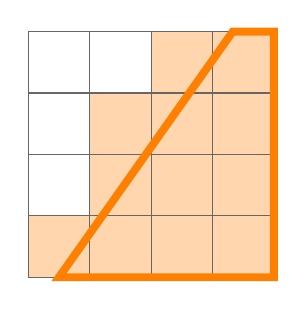
\begin{tikzpicture}[every node/.style={minimum size=0.6*1.3cm-\pgflinewidth, outer sep=0pt, fill=orange!80, fill opacity=0.4}, scale=0.6*1.3]
  \tikzmath{
    \gridheight=4;
    \gridwidth=4;
  }

  \def\cells{
    (0.5,0.5),
    (1.5,1.5),
    (2.5,2.5),
    (3.5,3.5),
    (3.5,2.5),
    (3.5,1.5),
    (3.5,0.5),
    (2.5,0.5),
    (1.5,0.5),
    (2.5,1.5),
    (2.5,3.5),
    (1.5,2.5)
  };
  \coordinate (offset) at (0.5, 0.5);
  \foreach \cell in \cells {
    \node at ($(\cell$) {};
  }

  \draw[step=1,color=black,draw opacity=0.6] (0,0) grid (\gridwidth,\gridheight);
  \draw[thick, orange, line width=0.1cm] (0.5, 0)
    -- (3.33, \gridheight)
    -- (\gridwidth, \gridheight)
    -- (\gridwidth, 0)
    -- cycle;
\end{tikzpicture}

  \hspace{2em}
  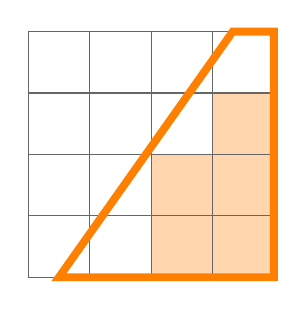
\begin{tikzpicture}[every node/.style={minimum size=0.6*1.3cm-\pgflinewidth, outer sep=0pt, fill=orange!80, fill opacity=0.4}, scale=0.6*1.3]
  \tikzmath{
    \gridheight=4;
    \gridwidth=4;
  }

  \def\cells{
    (3.5,2.5),
    (3.5,1.5),
    (3.5,0.5),
    (2.5,0.5),
    (2.5,1.5)
  };
  \coordinate (offset) at (0.5, 0.5);
  \foreach \cell in \cells {
    \node at ($(\cell$) {};
  }

  \draw[step=1,color=black,draw opacity=0.6] (0,0) grid (\gridwidth,\gridheight);
  \draw[thick, orange, line width=0.1cm] (0.5, 0)
    -- (3.33, \gridheight)
    -- (\gridwidth, \gridheight)
    -- (\gridwidth, 0)
    -- cycle;
\end{tikzpicture}

  \appcaption{%
    The same polygon discretized to a raster grid using two different techniques.
  }{%
    In the left figure, all pixels being \textit{touched} by the interior of the polygon
    are considered a part of the polygon (decision rule A), while in the left figure, only pixels
    entirely \textit{contained} within the interior are considered being part
    of the polygon (decision rule B).
  }%
  \label{fig:pixel-containment}
\end{figure}

\clearpage
An alternative is to average the two masks, resulting in mask values of $0.5$ where the two decision rules disagree.
Approximately \SI{9.2}{\percent} of mask pixels of value $1$ are situated along the boundary of a discretized mask polygon (\SI{1.7}{\percent} of \textit{all} pixels regardless of value) and may therefore be affected by this decision.
We have opted for decision rule B, as it has been observed to preserve symmetries and seams to a larger degree than decision rule A.
The distribution of the mask class balance across all produced tiles is shown in \cref{fig:mask-class-balance}.

\begin{figure}[H]
  \centering
  \includegraphics{mask-balance}
  \appcaption{%
    Distribution of \textit{building density} across all produced tiles in Trondheim.
  }{%
    Building density is defined by number of pixels positioned on top of buildings divided by total number of pixels.
  }%
  \label{fig:mask-class-balance}
\end{figure}

The average tile has a building density of approximately \SI{17}{\percent}, that is \SI{700}{\meter\squared} of \SI{4096}{\meter\squared} is occupied by buildings.
Of all the produced tiles approximately \SI{8.32}{\percent} end up having no positive mask pixels, i.e.\ no buildings are situated within these tiles.


\newpage
\section{Surface Rasterization Algorithm}%
\label{sec:surface-rasterization}
Let $r_{p,i}$ denote a linear ring belonging to a polygon denoted as $P_p$.
The symbol $p$ denotes the \textit{polygon index}, while $i$ denotes the \textit{ring index}.
A ring index of 1 indicates an \textit{exterior ring}, while a ring index of greater than one represents an interior ring.
The polygon $P_p$ can therefore be represented as a sequence of $|P_p| \geq 1$ linear rings,
%
\begin{equation*}
P_p = \{ r_{p,1}, \dots, r_{p, |P_p|}\}
\end{equation*}
%
Linear rings are represented as ordered sequences of $(x, y, z)$ coordinate tuples, assuming that the associated polygon is three-dimensional.
The linear ring can therefore be denoted as
%
\begin{equation*}
  r_{p,i}
  =
  \{
    (x_{p,i,1}, y_{p,i,1}, z_{p,i,1}),
    \dots,
    (x_{p,i,|r_{p, i}|}, y_{p,i,|r_{p, i}|}, z_{p,i,|r_{p, i}|}),
    (x_{p,i,1}, y_{p,i,1}, z_{p,i,1})
  \},
\end{equation*}
%
where the first and last coordinate tuple are identical in order to close the ring.
Now assume that the polygon collection at hand contains three-dimensional polygons which are all approximately planar.
Any $(x, y, z)$ vertex must therefore satisfy the following relationship:
%
\begin{equation*}
  z = \beta_{p,0} + \beta_{p,x} x + \beta_{p,y} y + \varepsilon
\end{equation*}
%
Where $\varepsilon$ is error term due to measurement errors or other type of random data errors.
The distribution of $\varepsilon$ must be investigated further for our dataset, but for the moment assume the error to be normally distributed with zero mean and some unknown variance $\sigma^2$, i.e. $\varepsilon \sim \mathcal{N}(0, \sigma^2)$.
%
The task is now to determine the coefficient vector $\vec{\beta}_p = {[\beta_{p,0}, \beta_{p,x}, \beta_{p,y}]}^T$ which describes the planar polygon surface.
We construct a design matrix $X_p$ consisting of all $(x, y)$ vertex coordinate tuples of the given polygon $P_p$:
%
\begin{equation*}
  X_p
  =
  \begin{bmatrix}
    1 & x_{p,1,1} & y_{p,1,1} \\
    1 & x_{p,1,2} & y_{p,1,2} \\
    \vdots & \vdots & \vdots \\
    1 & x_{p,1,|r_{p,1}|} & y_{p,1,|r_{p,1}|} \\
    1 & x_{p,2,1} & y_{p,2,1} \\
    1 & x_{p,2,2} & y_{p,2,2} \\
    \vdots & \vdots & \vdots \\
    1 & x_{p,|P_p|,|r_{|P_p|}|} & y_{p,|P_p|,|r_{|P_p|}|} \\
  \end{bmatrix}.
\end{equation*}
%
Likewise, a response vector $\vec{z}_p$ is constructed consisting of the respective elevation values associated with the $(x, y)$ tuples:
%
\begin{equation*}
  \vec{z}_p
  =
  \begin{bmatrix}
     z_{p,1,1} \\
     z_{p,1,2} \\
     \vdots \\
     z_{p,1,|r_{p,1}|} \\
     z_{p,2,1} \\
     z_{p,2,2} \\
     \vdots \\
     z_{p,|P_p|,|r_{|P_p|}|} \\
  \end{bmatrix}
\end{equation*}
%
Again, by assuming $\varepsilon \sim \mathcal{N}(0, \sigma^2)$ we construct an ordinary least squares estimator $\widehat{\vec{\beta}}_p $ for $\vec{\beta}_p$:
%
\begin{equation*}
  \widehat{\vec{\beta}}_p
  =
  {\left[
    \widehat{\beta}_{p,0},
    \widehat{\beta}_{p,x},
    \widehat{\beta}_{p,y}
  \right]}^T
  =
  \left( X_p^T X_p \right)^{-1} X_p^T \vec{z}_p
\end{equation*}
%
Interpolated elevation values for arbitrary $(x, y)$ coordinate tuples can now be constructed:
%
\begin{equation*}
  \widehat{z} = \widehat{\beta}_{p,0} + \widehat{\beta}_{p,x} x + \widehat{\beta}_{p,y} y
\end{equation*}
%
Or as an alternative formulation, a linear predictor $\widehat{f}_z$ parametrized according to $\widehat{\vec{\beta}}_p$ can be constructed:
%
\begin{equation*}
  \widehat{f}_z\left(x, y; \widehat{\vec{\beta}}_p\right)
  =
    \widehat{\beta}_{p,0}
    + \widehat{\beta}_{p,x} x
    + \widehat{\beta}_{p,y} y
  =
  \widehat{z}
\end{equation*}
%
Now define the coefficient vector set $\mathcal{B}(x, y)$ which contains all coefficient vectors to polygons that contain the coordinate $(x, y)$ when projected into the $xy$-plane.
More formally,
%
\begin{equation*}
  \mathcal{B}(x, y) = \left\{
    \vec{\beta}_p
    \mid
    (x, y) \in \pi_{\mathrm{2D}}(P_p)
  \right\},
\end{equation*}
%
where $\pi_{\mathrm{2D}}$ is the projection of all polygon vertex coordinates into the $xy$-plane as illustrated in \cref{fig:2d-polygon-projection}.
%
\begin{figure}
  \centering
  \includegraphics[width=\linewidth]{2d-projection}
  \caption{%
    Projection of three-dimensional polygon onto $xy$-plane by $\pi_{\mathrm{2D}}$.
  }{%
    The three-dimensional polygon is shown in \textcolor{red}{red}, while the two-dimensional projection is shown in \textcolor{blue}{blue}.
  }%
  \label{fig:2d-polygon-projection}
\end{figure}
%
\begin{equation*}
  \vec{\beta}_m(x, y)
  =
  \argmax_{\vec{\beta} \in \mathcal{B}(x, y)}
    \widehat{f}_z(x, y; \vec{\beta})
\end{equation*}
%
\begin{equation*}
  \vec{n}\left(\vec{\beta}\right)
  =
  \frac{%
    1
  }{%
    \sqrt{\beta_x^2 + \beta_y^2 + 1}
  }
  \cdot
  {\left[
    -\beta_{x}, -\beta_{y}, 1
  \right]}^T
\end{equation*}


\begin{figure}
  \centering
  \includegraphics[width=\linewidth]{interpolation-concepts}
  \caption{Three-dimensional surface raster values}{%
    Illustration of interpolated altitude values, $Z_{ij}$, and respective surface normal vectors, $N_{ij}$.
    Slice for $i = 1$ and $1 \leq j \leq 4$.
  }
\end{figure}

\begin{algorithm}{Surface interpolation}{alg:surface-interpolation}{Tile bounding box $B(\vec{c}, w, h)$,\\Raster dimensions $H \times W$,\\R-Tree indexed polygon collection.}
\item Construct arrays with temporary placeholder values:
  \begin{itemize}[label=--,leftmargin=0cm]
    \item Normal vector array $N$ of size $H \times W \times 3$ filled with $0$.
    \item Interpolated elevation array $Z$ of size $H \times W \times 1$ filled with $-\infty$.
  \end{itemize}
\item Construct polygon collection $\mathcal{P}$ for given tile extents using R-Tree index.
  Convert polygons to pixel coordinate system.
\item For polygon $P_p = [r_{p0}, r_{p1}, \dots, r_{pn_p}]$ with a single exterior ring, $r_{p0}$, and $n_p$ interior rings, $[r_{p1}, \ldots, r_{pn_p}]$, in polygon collection $\mathcal{P}$.
  \begin{enumerate}[leftmargin=0.5em,label=\textbf{\alph*}]
      % \item The linear ring $r_{pj} = [(x_{pj0}, y_{pj0}, z_{ij0}), \dots, (x_{pjn_{ij}}, y_{ijn_{pj}}, z_{ijn_{pj}})]$.
    \item Construct $M \times 3$ design matrix $X$ populated with pixel coordinates of all \textit{unique} xy-vertices $(1, x_{pij}, y_{pij})$.
        Secondly, construct $M \times 1$ response vector $\vec{y}$ populated with the respective $z_{pij}$ coordinates.
    \item Solve linear regression problem $\vec{\beta}_p = {\left(\beta_0, \beta_x, \beta_y\right)}^T = {\left(X^T X\right)}^{-1} X^T \vec{y}$
    \item Construct polygon surface normal vector $\vec{n}_p$,
      \begin{equation*}
        \vec{n}_p \assign {\left(\beta_x^2 + \beta_y^2 + 1\right)}^{-1/2} \cdot {\left(-\beta_x, -\beta_y, 1\right)}^T,
      \end{equation*}
      where $||\vec{n}_p||_2 = 1$ by construction.
    \item For each pixel coordinate $(i, j)$ contained by the polygon $P_p$ projected onto the 2-dimensional pixel index plane:
      \begin{itemize}[leftmargin=0.5em]
        \item $h \assign \beta_0 + \beta_x j + \beta_y i$. If $h < Z_ij$, continue loop, else\dots
        \item $Z_{ij} \assign h$ and $\left(N_{ijx}, N_{ijy}, N_{ijz}\right) \assign \vec{n}_p$.
      \end{itemize}
    \end{enumerate}
\end{algorithm}


\chapter{Modelling}%
\label{sec:modeling}
The field of \textit{computer vision} got started in the early 1970s~\cite[p.~10]{computer_vision_history}, where one of the problems being tackled is the three-dimensional reconstruction of a scene from two-dimensional data.
Most of the early research in the field revolved around manually designed feature extraction and processing techniques, but statistical techniques started to become popular in the 1990s~\cite[p.~15]{computer_vision_history}.
The statistical approach eventually morphed into the field of \textit{machine learning}, where most of the research advances are made today~\cite[p.~17]{computer_vision_history}.

We have already provided an overview of the problem domains of interest in \cref{sec:segmentation-description}, but we will now provide a more in-depth description of all the relevant theoretical concepts.
\textit{Convolutional neural networks} (CNNs) have been applied to image segmentation problems with great success~\cite[p.~1]{image_recognition}, and \cref{sec:cnn} provides a theoretic overview of the elementary building blocks used to construct modern CNN architectures.
\Cref{sec:semantic-segmentation} will summarize the metrics used for evaluating the quality of image segmentation predictions.
State-of-the-art CNN architectures for image segmentation will be listed in \cref{sec:segmentation-state-of-the-art}.


\section{Convolutional Neural Networks (CNNs)}%
\label{sec:cnn}
There exists countless variations of the CNN model architecture, but there are still some elementary building blocks which they often have in common.
We will start by sketching generic big picture of CNNs before going into detail about each modular building block.
\Cref{fig:unet} illustrates the architecture of \textit{U-Net}, and we will use this figure to illustrate the common concepts of segmentation CNNs without considering the unique properties of U-Net specifically.

\begin{figure}[H]
  \includegraphics[width=\textwidth]{unet}
  \appcaption{%
    Illustration of the U-Net architecture for single-class segmentation, a typical example of an \textit{encoder/decoder} structure.
  }{%
    Convolution layers are shown in orange, and max pooling layers in red.
    Arrows indicates how data is forwarded through the network, top arrows being \textit{skip connections}.
    The right hand side shows the upscaling performed by \textit{transposed convolution} until the original resolution is restored and segmentation predictions can be formed with the \textit{sigmoid} activation function (shown in purple).
    Figure has been generated by modifying a \texttt{tikz} example provided in the MIT licenced \texttt{PlotNeuralNet} library available at this URL:\@
    \protect\url{https://github.com/HarisIqbal88/PlotNeuralNet}.
  }%
  \label{fig:unet}
\end{figure}

A CNN consists of several layered blocks operating over identical input dimensions within each block.
These blocks are shown as contiguous boxes in \cref{fig:unet}.
The first layer in each block is a \textit{convolutional layer}, which is a type of trainable feature extraction where several filtered \textit{feature maps} are constructed.
Each feature map is passed through a nonlinear \textit{activation function} and the \textit{activations} are subsequently downsampled in order to reduce the resolution.
The downsampling is performed by a \textit{pooling layer} and the output is forwarded to the next block.
The number of feature maps that are extracted from the previous pooled activations increases as the resolution is decreased, and the right half of the architecture is eventually responsible for upsampling the resolution back to the original resolution by the means of \textit{deconvolution}.
The upsampling half of this network is not common to all CNNs, as CNNs tasked with bounding box regression and classification are not required to restore the original resolution before prediction.
The upcoming sections will describe these concepts in more detail.

\subsection{Convolution}
As the name implies, a central concept of convolutional neural networks is the \textit{convolution operator}.
Let the \textit{kernel}, $w$, be a $H_k \times W_k$ real matrix, and denote the activation of the previous layer at position $(x, y)$ as $a_{x, y}$.
The \textit{convolution operator}, $\circledast$, is then defined as
%
\begin{align*}
  w \circledast a_{x, y} = \sum_{i} \sum_{j} w_{i, j} ~ a_{x - i, y - j},
  \hspace{3em}
    a_{x, y} \in \mathbb{R},~
    w \in \mathbb{R}^{H_k \times W_k},
\end{align*}
%
where $(i, j)$ spans the index set of the kernel.
The region around $a_{x,y}$ which is involved in the convolution is referred to as the \textit{receptive field}.
We can generate a \textit{filtered image} by moving this receptive field over the entire input image.
The step size used when moving the receptive field is referred to as the \textit{stride size} of the convolution.
Such a \textit{moving convolution} is illustrated in \cref{fig:convolution}.

\begin{figure}[H]
  %%%%%%%%%%%%%%%%%%% Local functions %%%%%%%%%%%%%%%%%%%
%% -- Draw marks
\newbox\dumbox% chktex 1
\newcommand{\mymark}[2]{%
  \setbox\dumbox=\hbox{#2}%
  \hbox to \wd\dumbox{\hss% chktex 1
    \tikz[overlay,remember picture,baseline=(#1.base)]{ \node (#1) {\box\dumbox}; }% chktex 36
    \hss}%
}

%%%%%%%%%%%%%%%%%%% Local functions %%%%%%%%%%%%%%%%%%%

\[
\underbracket[0.6pt][7pt]{
\left[\begin{array}{ccccccc}
  \mymark{TL3}{0} & 0 & 0 & 0 & 0 & \mymark{TR3}{0} \\
  0 & 1 & \mymark{TL1}{2} & 0 & \mymark{TR1}{0} & 0 \\
  0 & 5 & 3 &               0 & 4 &               0 \\
  0 & 0 & \mymark{BL1}{0} & 0 & \mymark{BR1}{7} & 0 \\
  0 & 9 & 3 & 0 & 0 & 0 \\
  \mymark{BL3}{0} & 0 & 0 & 0 & 0 & \mymark{BR3}{0} \\
\end{array}\right]
}_{\text{Zero-padded input}}
*
\underbracket[0.6pt][7pt]{
\left[\begin{array}{ccc}
  \mymark{TL2}{1} & 1 & \mymark{TR2}{1}\\
  1  & 1 &              0 \\
  \mymark{BL2}{1} & 0 & \mymark{BR2}{0}
\end{array}\right]
}_{\text{Kernel}}
=
\underbracket[0.6pt][7pt]{
\left[\begin{array}{ccccccc}
  1 & 8 & 5 & 0 \\
  8 & 11 & \mymark{C}{5} & 4 \\
  8 & 17 & 10 & 11 \\
  9 & 12 & 10 & 7 \\
\end{array}\right]
}_{\text{Convolved output}}
\]

\begin{tikzpicture}[overlay, remember picture,
    myedge1/.style={thin, opacity=.3, blue},
    myedge2/.style={thin, opacity=.3, green!40!black}]

  %% Draw boxes
  \draw[orange, fill=orange, fill opacity=.1]   (TL1.north west) rectangle (BR1.south east);
  \draw[blue, fill=blue, fill opacity=.1] (TL2.north west) rectangle (BR2.south east);
  \draw[green!60!black, fill=green, fill opacity=.1] (C.north west) rectangle (C.south east);

  %% Draw blue lines
  \draw[myedge1] (TL1.north west) -- (TL2.north west);
  \draw[myedge1] (BL1.south west) -- (BL2.south west);
  \draw[myedge1] (TR1.north east) -- (TR2.north east);
  \draw[myedge1] (BR1.south east) -- (BR2.south east);

  %% Draw green lines
  \draw[myedge2] (TL2.north west) -- (C.north west);
  \draw[myedge2] (BL2.south west) -- (C.south west);
  \draw[myedge2] (TR2.north east) -- (C.north east);
  \draw[myedge2] (BR2.south east) -- (C.south east);

  \fill[gray, fill opacity = 0.1, even odd rule]
    (TL3.north west) rectangle (BR3.south east)
    (TL3.south east) rectangle (BR3.north west);
\end{tikzpicture}

  \caption[Visualization of a kernel convolution.]{
    Visualization of a kernel convolution with a $3 \times 3$ kernel over an image of size $4 \times 4$ with additional zero-padding and stride size of $1 \times 1$.
    The \textit{receptive field} is shown in \textcolor{orange}{orange}, the respective kernel weights in \textcolor{blue}{blue}, and the resulting convolution output in \textcolor{green}{green}.
    The zero padding of the input image is shown in gray.
  }%
  \label{fig:convolution}
\end{figure}

In the case of input images or activations comprised of more than one channel, independent two-dimensional kernels are constructed for each channel and the convolved outputs are finally summed in order to attain a single feature map.
The concept of a \textit{kernel} predates neural networks as it has been used for feature extraction in the field of image processing for many years~\cite[p.~11]{computer_vision_history}.
The kernel weights determine the type of features being extracted from the given input image, some common interpretable kernels are given below.

\begin{footnotesize}\begin{align*}
  \underbracket[0.6pt][7pt]{
    w_1 =
    \begin{bmatrix}
      0 & 0 & 0 \\
      0 & 1 & 0 \\
      0 & 0 & 0 \\
    \end{bmatrix}
  }_{\text{Identity kernel}},
  &&
  \underbracket[0.6pt][7pt]{
    w_2 =
    \begin{bmatrix}
      -1 & -1 & -1 \\
      -1 & 8 & -1 \\
      -1 & -1 & -1 \\
    \end{bmatrix}
  }_{\text{Edge detection kernel}},
  &&
  \underbracket[0.6pt][7pt]{
    w_3 =
    \frac{1}{9}
    \begin{bmatrix}
      1 & 1 & 1 \\
      1 & 1 & 1 \\
      1 & 1 & 1 \\
    \end{bmatrix}
  }_{\text{Normalized box blur kernel}},
  &&
  \underbracket[0.6pt][7pt]{
    w_4 =
    \frac{1}{16}
    \begin{bmatrix}
      1 & 2 & 1 \\
      2 & 4 & 2 \\
      1 & 2 & 1 \\
    \end{bmatrix}
  }_{\text{Gaussian blur kernel}}.
\end{align*}\end{footnotesize}

It is important to notice that kernel convolution has the additional effect of reducing the dimensionality of the input image.
Firstly, pixels along the image border are partially ignored since the receptive field can not be properly centered on these pixel.
Secondly, a horizontal stride of $W_s > 1$ or a vertical stride of $H_s > 1$ will cause additional dimensional reduction.
For an image of size $H \times W$ and a kernel of size $H_k \times W_k$, the input image is reduced to size
%
\begin{equation*}
  \floor{(H - H_k + H_s) / H_s}
  \times
  \floor{(W - W_k + W_s) / W_s}.
\end{equation*}
%
as shown by~\cite{dive-into-deep-learning}.
The reduction in dimensionality when using stride sizes of one is often undesirable, and for this reason it is common to add a \textit{padding} filled with zero-values along the edges of the input image.
Applying a padding of height $H_p$ at the horizontal borders and a padding of width $W_p$ at the vertical borders results in a feature map of size
%
\begin{equation*}
  \floor{(H - H_k + H_s + \mathbf{H_p}) / H_s}
  \times
  \floor{(W - W_k + W_s + \mathbf{W_p}) / W_s}.
\end{equation*}
%
If we assume the input height and width to be divisible by the stride height and width respectively, we can set $H_p = H_k - 1$ and $W_p = W_k - 1$ in order to attain an output shape of $(H / H_s) \times (W / W_s)$~\cite{dive-into-deep-learning}.
Such a padding is shown in gray in \cref{fig:convolution}.

CNNs apply multiple different convolutions to the same input, resulting in a set of differently filtered outputs.
After having applied the layer's activation function to the output (see upcoming section about \enquote{activation functions}) and the activations have been downsampled (see upcoming \enquote{pooling} section), the filtered outputs are passed onto the next layer.
The number of filters are usually increased as you move deeper into the network where the resolution has been increasingly downsampled.
Unlike classical image processing, where kernel weights are carefully selected in order to construct an intended type of feature extraction, CNNs let each kernel weight be a trainable parameter.
As the network is trained each kernel learns to extract features which are of use for the subsequent layers.

An important aspect of convolution is that the kernel weights remain unchanged as the receptive field is moved over the input image.
This \textit{parameter sharing} results in regions being treated identically no matter where in the image they are situated~\cite{visint-cnn}.
The sharing of parameters has the benefit of reducing the parametric complexity of the network, thus decreasing the computational cost of training it.
Finally, compared to a more classical \textit{fully connected feedforward network}, which operates over flattened vectors, a fully convolutional neural network operates over images in matrix form, thus taking the spatial relationship between pixels into account.

\subsection{Activation functions}
So far we have only explained how a convolutional neural network consists of a set of parametrized linear operations.
Such a network, if left unaltered, is therefore restricted to only approximating linear functions.
The solution to this predicament is to introduce the concept of an \textit{activation function}, a nonlinear function applied to the output from the convolutional layers.
These activation functions were originally inspired by the neuroscientific understanding of biological neurons~\cite[p.~165]{goodfellow}, but have since been shown to be a theoretical prerequisite of the \textit{universal approximation} property of artificial neural networks~\cite{uat-sigmoid,uat-nonpolynomial}.
The \textit{logistic sigmoid} function, with its deep roots in probability theory, has been a popular choice of activation function for neural networks since the inception of the field~\cite{rosenblatt-perceptron-1958}, and is defined by
%
\begin{equation*}
  \sigma(x) = \frac{1}{1 + e^{-x}} = \frac{e^x}{e^x + 1}.
  \tag{Sigmoid activation function}
\end{equation*}
%
Observe that $\lim_{x \to -\infty} \sigma(x) = 0$ and $\lim_{x \to +\infty} \sigma(x) = 1$, and that its derivative is positive over the entire real number line. This makes it a bounded, differentiable, monotonic function, and is therefore suitable for mapping the weighted output of an artificial neuron in the domain $(-\infty, \infty)$ into the range $(0, 1)$.
This makes it especially suitable for the final layer in neural networks intended for predicting binary 0/1-responses.

Although the sigmoid activation function has strong biological~\cite{rosenblatt-perceptron-1958} and theoretical~\cite{uat-sigmoid} underpinnings, it often suffers from the phenomenon of \textit{vanishing gradients} for network architectures consisting of three or more layers, which in turn severely inhibits training.
As an alternative to the sigmoid activation function, the \textit{rectified linear unit} (ReLU) was introduced in a paper~\cite{relu-original-paper} by \citeauthor{relu-original-paper} in year \citeyear{relu-original-paper}.
It is defined as
%
\begin{equation*}
  \mathrm{ReLU}(x) = x^+ = \max(0, x).
  \tag{ReLU activation function}
\end{equation*}
%
The ReLU activation function has become the dominant activation function for use in neural networks in recent years~\cite[p.~438]{relu-popularity} as it has been empirically shown to adapt well to deeper neural networks~\cite{relu-better-than-sigmoid}.

\subsection{Pooling}
The last layer in a given CNN block is conventionally a \textit{downsampling} operation, most often referred to as a \textit{pooling} layer.
As with convolution, this operation has biological influences as it is inspired by a model of the mammalian visual cortex~\cite[p.~966]{visint-cnn}.
The reduction in spatial resolution is considered to be one of the main reasons for why CNNs portray a high degree of translational and rotational invariance~\cite{cnn-translational-invariance}.
As with moving convolution, pooling is implemented by moving a receptive field of size greater than $1$, typically $2 \times 2$, over the activations and mapping these values into a lower dimensional space.
There are several different ways to define such a mapping, the two most common being \textit{max pooling} and \textit{average pooling}, which respectively retrieve the maximum value and average value from the receptive field.
The former is exemplified in \cref{fig:max-pooling}.

\begin{figure}[H]
  %%%%%%%%%%%%%%%%%%% Local functions %%%%%%%%%%%%%%%%%%%
%% -- Draw marks
\newbox\dumbox% chktex 1
\newcommand{\mymark}[2]{%
  \setbox\dumbox=\hbox{#2}%
  \hbox to \wd\dumbox{\hss% chktex 1
    \tikz[overlay,remember picture,baseline=(#1.base)]{\node (#1) {\box\dumbox};}% chktex 36
    \hss}%
}

%%%%%%%%%%%%%%%%%%% Local functions %%%%%%%%%%%%%%%%%%%

\[
\underbracket[0.6pt][7pt]{
\left[\begin{array}{cccc}
  1 & 8 & \mymark{TL1}{5} & \mymark{TR1}{0} \\
  8 & 11 & \mymark{BL1}{5} & \mymark{BR1}{4} \\
  8 & 17 &               10 & 11               \\
  9 & 12 & 10 & 7 \\
\end{array}\right]
}_{\text{Activations}}
\hspace{0.5em}
\underbracket[0.6pt][7pt]{
\begin{array}{ccc}
    \mymark{TL2}{\phantom{1}} & \phantom{1} & \mymark{TR2}{\phantom{1}}\\
    \phantom{1}  & \mymark{mycenter}{\phantom{1}} &              \phantom{0} \\
    \mymark{BL2}{\phantom{1}} & \phantom{0} & \mymark{BR2}{\phantom{0}}
\end{array}
}_{\text{Pool operation}}
=
\underbracket[0.6pt][7pt]{
\left[\begin{array}{cccccc}
  11 & \mymark{C}{5} \\
  17 & 11 \\
\end{array}\right]
}_{\text{Pooled output}}
\]

\begin{tikzpicture}[overlay, remember picture,
    myedge1/.style={thin, opacity=.3, blue},
    myedge2/.style={thin, opacity=.3, green!40!black}]

  %% Draw boxes
  \draw[orange, fill=orange, fill opacity=.1]   (TL1.north west) rectangle (BR1.south east);
  \draw[blue, fill=blue, fill opacity=.1] (TL2.north west) rectangle (BR2.south east)
    node[midway, opacity=1, color=black] {\Large $\max$};
  \draw[green!60!black, fill=green, fill opacity=.1] (C.north west) rectangle (C.south east);

  %% Draw blue lines
  \draw[myedge1] (TL1.north west) -- (TL2.north west);
  \draw[myedge1] (BL1.south west) -- (BL2.south west);
  \draw[myedge1] (TR1.north east) -- (TR2.north east);
  \draw[myedge1] (BR1.south east) -- (BR2.south east);

  %% Draw green lines
  \draw[myedge2] (TL2.north west) -- (C.north west);
  \draw[myedge2] (BL2.south west) -- (C.south west);
  \draw[myedge2] (TR2.north east) -- (C.north east);
  \draw[myedge2] (BR2.south east) -- (C.south east);
\end{tikzpicture}

  \appcaption{%
    Example of a \textit{max-pooling} operation with a receptive field of size $2 \times 2$ and an identical stride size.
  }{%
    The receptive field is shown in \textcolor{orange}{orange} and the respective pooled output is shown in \textcolor{green}{green}.
  }%
  \label{fig:max-pooling}
\end{figure}

As can be seen in \cref{fig:max-pooling}, using a receptive field and stride of size $2 \times 2$ will yield a downsampled image with one quarter as many pixels as the original input.

\subsection{Batch normalization}
The reparametrization of earlier layers when training deep neural networks results in a distributional change in the feature layer forwarded to the next layers.
This forces all subsequent layers to adapt to the new \enquote{distributional circumstances}, which in turn impedes the convergence of the optimization.
This phenomenon, referred to as \textit{internal covariate shift}, was first identified in a paper~\cite{batch-normalization} by \citeauthor{batch-normalization}~(\citeyear{batch-normalization}) where they propose a method called \textit{batch normalization} in order to counter this phenomenon.
Suppose we have a layer activation $\vec{a}$ consisting of $d$ dimensions, i.e. $\vec{a} = (a^{(1)}, \ldots, a^{(d)})$.
First we standardize each feature dimension, $k$, independently

\begin{equation*}
  \widehat{a}^{(k)}
  =
  \frac{
    a^{(k)} - \E{a^{(k)}}
  }{
    \sqrt{\Var{a^{(k)}} + \epsilon}
  },
  \tag{Batch standardization}
\end{equation*}

where $\E{\cdot}$ and $\Var{\cdot}$ are respectively sample means and sample variances over the current mini-batch, and $\epsilon$ is added for numerical stability.
The result of this standardization is a feature map where all filters have mean $0$ and variance $1$ for every mini-batch.
The internal covariate shift has been practically eliminated as a result.

This type of normalization alone may not be optimal in all cases, though, and is best explained by constructing a somewhat contrived pathological example.
Assume a set of pooled layer activations $\vec{a}$ to be symmetrically distributed, and assume the subsequent convolution layer to preserve this symmetry.
After standardizing the output, 50\% of the values are expected to be negative, and all of these values will be truncated to $0$ if ReLU is the activation function of choice.
This informational loss may be suboptimal for the given network layer and must be accounted for.
That is to say, $\E{a} =  0$ and $\Var{a}$ may be an unsuitable domain for the given activation function.
For this reason, we introduce two additional trainable parameters for each feature dimension, $\gamma^{(k)}$ and $\beta^{(k)}$, and apply a second normalization step

\begin{equation*}
  y^{(k)} = \gamma^{(k)} \widehat{a}^{(k)} + \beta^{(k)}.
  \tag{Trainable normalization}
\end{equation*}

The intent is to learn the values for the shift, $\beta^{(k)}$, and scaler, $\gamma^{(k)}$, which restores the representative power of the given layer \textit{after} the batch standardization.

\subsection{Dropout}
Dropout is a regularization technique for neural networks intended to prevent \enquote{complex co-adaption of feature detectors}~\cite{dropout-original-paper}.
In practice this is achieved by randomly omitting hidden nodes from the neural network during each training step; effectively forcing hidden nodes to become less interdependent.
An alternative interpretation of the dropout procedure is that it is a computationally efficient form of model averaging, each dropout permutation being a model instance.
This technique has been empirically shown to significantly increase the test performance in several different settings.

Although originally intended for use in feedforward neural networks, dropout has been extensively applied in CNN architectures as well~\cite{dropout-cnn}.
Since there are no nodes to be omitted in fully convolutional layers, the dropout procedure needs to be adapted in order to be applicable in a CNN setting.
One approach is to introduce a randomly located square mask (\textit{cutout}) in the input image~\cite{dropout-cutout}.
\textit{Stochastic depth dropout} randomly selects entire layers to be dropped, replacing them with identity functions instead~\cite{dropout-stochastic-depth}.
Dropout can also be integrated into max pooling layers, ignoring values at random during the search for the maximum value in the receptive field~\cite{max-pooling-dropout}.
This has become known as \textit{max-pooling dropout} and is illustrated in \cref{fig:max-pooling-dropout}.

\begin{figure}[H]
  %%%%%%%%%%%%%%%%%%% Local functions %%%%%%%%%%%%%%%%%%%
%% -- Draw marks
\newbox\dumbox% chktex 1
\newcommand{\mymark}[2]{%
  \setbox\dumbox=\hbox{#2}%
  \hbox to \wd\dumbox{\hss% chktex 1
    \tikz[overlay,remember picture,baseline=(#1.base)]{\node (#1) {\box\dumbox};}% chktex 36
    \hss}%
}
% Used to indicate dropout array indices
\newcommand{\dropout}[1]{{\setlength{\fboxsep}{0pt}\fcolorbox{black}{black}{#1}}}

%%%%%%%%%%%%%%%%%%% Local functions %%%%%%%%%%%%%%%%%%%

\begin{align*}
  \left[\begin{array}{cccc}
    1 & 8 & \mymark{oldTL1}{5} & \mymark{oldTR1}{0} \\
    8 & 11 & \mymark{oldBL1}{5} & \mymark{oldBR1}{4} \\
    8 & 17 &               10 & 11               \\
    9 & \mymark{old}{12} & 10 & 7 \\
  \end{array}\right]
  \hspace{0.5em}
  \begin{array}{ccc}
      \mymark{oldTL2}{\phantom{1}} & \phantom{1} & \mymark{oldTR2}{\phantom{1}}\\
      \phantom{1}  & \mymark{oldmycenter}{\phantom{1}} &              \phantom{0} \\
      \mymark{oldBL2}{\phantom{1}} & \phantom{0} & \mymark{oldBR2}{\phantom{0}}
  \end{array}
  =
  \left[\begin{array}{cccccc}
    11 & \mymark{oldC}{5} \\
    17 & 11 \\
  \end{array}\right]
  \\[2.25em]
  \left[\begin{array}{cccc}
    1 & \mymark{new}{8} & \mymark{TL1}{\dropout{5}} & \mymark{TR1}{0} \\
    \dropout{8} & 11 & \mymark{BL1}{\dropout{5}} & \mymark{BR1}{4} \\
    8 & \dropout{1} &               10 & 11               \\
    \dropout{9} & 12 & 10 & 7 \\
  \end{array}\right]
  \hspace{0.5em}
  \begin{array}{ccc}
      \mymark{TL2}{\phantom{1}} & \phantom{1} & \mymark{TR2}{\phantom{1}}\\
      \phantom{1}  & \mymark{mycenter}{\phantom{1}} &              \phantom{0} \\
      \mymark{BL2}{\phantom{1}} & \phantom{0} & \mymark{BR2}{\phantom{0}}
  \end{array}
  =
  \left[\begin{array}{cccccc}
    11 & \mymark{C}{4} \\
    12 & 11 \\
  \end{array}\right]
\end{align*}

\begin{tikzpicture}[overlay, remember picture,
    myedge1/.style={thin, opacity=.3, blue},
    myedge2/.style={thin, opacity=.3, green!40!black}]

  %% Draw boxes
  \draw[orange, fill=orange, fill opacity=.1]   (TL1.north west) rectangle (BR1.south east);
  \draw[orange, fill=orange, fill opacity=.1]   (oldTL1.north west) rectangle (oldBR1.south east);

  \draw[blue, fill=blue, fill opacity=.1] (TL2.north west) rectangle (BR2.south east)
    node[midway, opacity=1, color=black] {\Large $\max$};
  \draw[blue, fill=blue, fill opacity=.1] (oldTL2.north west) rectangle (oldBR2.south east)
    node[midway, opacity=1, color=black] {\Large $\max$};

  \draw[green!60!black, fill=green, fill opacity=.1] (C.north west) rectangle (C.south east);
  \draw[green!60!black, fill=green, fill opacity=.1] (oldC.north west) rectangle (oldC.south east);

  %% Draw blue lines
  \draw[myedge1] (TL1.north west) -- (TL2.north west);
  \draw[myedge1] (BL1.south west) -- (BL2.south west);
  \draw[myedge1] (TR1.north east) -- (TR2.north east);
  \draw[myedge1] (BR1.south east) -- (BR2.south east);
  \draw[myedge1] (oldTL1.north west) -- (oldTL2.north west);
  \draw[myedge1] (oldBL1.south west) -- (oldBL2.south west);
  \draw[myedge1] (oldTR1.north east) -- (oldTR2.north east);
  \draw[myedge1] (oldBR1.south east) -- (oldBR2.south east);

  %% Draw green lines
  \draw[myedge2] (TL2.north west) -- (C.north west);
  \draw[myedge2] (BL2.south west) -- (C.south west);
  \draw[myedge2] (TR2.north east) -- (C.north east);
  \draw[myedge2] (BR2.south east) -- (C.south east);
  \draw[myedge2] (oldTL2.north west) -- (oldC.north west);
  \draw[myedge2] (oldBL2.south west) -- (oldC.south west);
  \draw[myedge2] (oldTR2.north east) -- (oldC.north east);
  \draw[myedge2] (oldBR2.south east) -- (oldC.south east);

  % Draw arrow from old to new activation matrix
  \draw[->, line width=0.5mm, shorten >= 2mm] (old) ++ (-0.1mm, -4mm) -- node[auto, yshift=1mm] {Dropout} (new.north);
\end{tikzpicture}

  \caption{%
    An example application of \textit{max-pooling dropout} using a receptive field and stride of size $2 \times 2$.
    A dropout probability of $p = 0.25$ has been used.
    Dropped values are shown as black boxes.
  }%
  \label{fig:max-pooling-dropout}
\end{figure}



\section{Semantic Segmentation}%
\label{sec:semantic-segmentation}
\todo{Make this introduction make sense after not only being about metrics, losses, and optimization.}
Metrics and losses are of central importance when training and evaluating machine learning models.
Denote the parametrization of a given machine learning model, $\hat{f}$, as $\vec{\theta}$, the input features as $X$, and the corresponding \textit{ground truth} labels as $Y$.
In order to evaluate the performance of a given model parametrization, we must formulate a cost- or performance-\textit{metric}, $P(\hat{f}(X; \theta); Y)$, which we intend to respectively minimize or maximize.
The performance metric encodes our notion of what constitutes as a good model fit.

While the performance metric is what we really want to optimize, it may not be suitable for numerical optimization, for example due to being non-differentiable or too computationally costly.
Machine learning optimization differs from classical optimization in that the performance metric is indirectly maximized through the optimization of a surrogate \textit{loss} function~\cite[p.~272]{goodfellow}, $\mathcal{L}(\hat{f}(X; \vec{\theta});  Y)$.
The loss metric is minimized in the hope of improving the performance metric indirectly, and it is therefore of vital importance that there is a strong relationship between performing well on the loss function and performing well on the performance metric.

We will provide a summary of popular losses and metrics for single-class semantic segmentation.

\subsection{Accuracy, sensitivity, and specificity}
In order to describe segmentation metrics, it is useful to define the following quantities:

\begin{center}
  \fbox{%
    \parbox{0.9\linewidth}{%
      \begin{description}[leftmargin=1cm, before={\renewcommand\makelabel[1]{\bfseries ##1:}}]
        \item[Condition Positive (P)]
          Number of object class pixels in ground truth mask.
        \item[Condition Negative (N)]
          Number of non-object class pixels in ground truth mask.
        \item[True Positive (TP)]
          Number of pixels correctly predicted as being part of object class (correctly identified).
        \item[True Negative (TN)]
          Number of pixels correctly predicted as \textit{not} being part of object class (correctly rejected).
        \item[False Positive (FP)]
          Number of pixel incorrectly predicted as being part of object class (incorrectly identified).
        \item[False Negative (FN)]
          Number of pixel incorrectly predicted as \textit{not} being part of object class (incorrectly rejected).
      \end{description}
    }
  }
\end{center}

False positives (FP) are often knows as \textit{type I errors} in statistics, and false negatives (FN) as \textit{Type II errors}.
The greater the values of TP and TN, the better, and the smaller the values of FP and FN, the better.
A visual representation of these classifications is given in \cref{fig:confusions}.

\begin{figure}[H]
  \includegraphics[width=\linewidth]{confusions}
  \caption[Illustration of TP, TN, FP, and FN for a binary segmentation prediction.]{%
    Binary segmentation problem of size $256 \times 256$.
    The ground truth, a rectangle of size $120 \times 80$ is shown on the left.
    The \enquote{predicted} mask, shown in the middle, is of the same size, but offset by $(-30, -30)$.
    The right figure shows the visual equivalent of a confusion matrix.
    True positives are shown in \textcolor{tp}{dark blue}, true negatives in \textcolor{gray}{light gray}, false positives in \textcolor{fp}{green}, and false negatives in \textcolor{fn}{red}.
  }%
  \label{fig:confusions}
\end{figure}

The simplest metric for semantic segmentation is the \textit{pixel accuracy} metric.
This metric simply reports the percentage of pixels that were correctly classified.
More formally, it can be defined as:

\begin{equation*}
    \textbf{accuracy} = \frac{TP + TN}{TP + TN + FP + FN} = \frac{TP + TN}{P + N}
\end{equation*}

The problem with the pixel-wise accuracy metric is that it does not take class imbalances into account.
Consider a problem where 95\% of all pixels are considered to be of class $0$, and the remaining 5\% of class $1$.
If we construct a model which predicts $0$ regardless of the feature inputs provided to the model, the model will achieve a 95\% accuracy score.
This makes pixel-wise accuracy scores hard to interpret when you do not know the class balance of the respective dataset and the accuracy grouped by class.
This is why it is often replaced by other metrics which take imbalances into account.
A pair of such metrics are \textit{sensitivity} and \textit{specificity}, formally defined as:

\begin{small}
\begin{align*}
    \textbf{sensitivity}
    &=
    \frac{\text{number of true positives}}{\text{number of true positives + number of false negatives}}
    =
    \frac{TP}{TP + FN}
    =
    \frac{TP}{P}
    \\
    \textbf{specificity}
    &=
    \frac{\text{number of true negatives}}{\text{number of true negatives + number of false positives}}
    =
    \frac{TN}{TN + FP}
    =
    \frac{TN}{N}
\end{align*}
\end{small}

The \textit{sensitivity} is therefore a measure of how good a given model prediction is able to identify positives as a relative, fractional value.
Likewise, the \textit{specificity} is a measure of how good a given model prediction is able to identify negatives.

\subsection{Intersection over union and dice coefficient}
Although the sensitivity and specificity metrics address the issue of class imbalances, they are still \textit{two} distinct metrics that need to be simultaneously inspected in order to get a full overview of the model performance.
Is it possible to construct a \textit{single} scalar metric which incorporates the ideas of both sensitivity and specificity?
The \textit{intersection over union} (IoU) and \textit{dice coefficient} ($F_1$) are two metrics which try to do exactly this.

The IoU metric, also known as the \textit{Jaccard index}, is defined as the area of the intersection between the predicted segmentation mask and the ground truth mask divided by the union of these two masks, or more formally,
%
\begin{equation*}
  \mathrm{IoU}
  =
  \frac{%
    |\mathrm{prediction} \cap \mathrm{truth}|
  }{%
    |\mathrm{prediction} \cup \mathrm{truth}|
  }
  =
  \frac{%
    \mathrm{TP}
  }{%
    \mathrm{TP} + \mathrm{FP} + \mathrm{FN}
  }.
\end{equation*}
%
In the case of multiple classes IoU is calculated for each class independently and the result is averaged, known as \textit{mean intersection over union} (MIoU).
MIoU is the most commonly used segmentation metric in research and competitions due to its simplicity and representativeness~\cite{segmentation-overview}.
Notice how the IoU metric is bounded between 0 and 1; $\mathrm{IoU} = 0$ represents a complete \enquote{predictive miss}, while $\mathrm{IoU} = 1$ represents a prediction in perfect accordance with the ground truth.
A visualization of this metric is given in \cref{fig:iou-metric} below.

\begin{figure}[H]
  \centering
  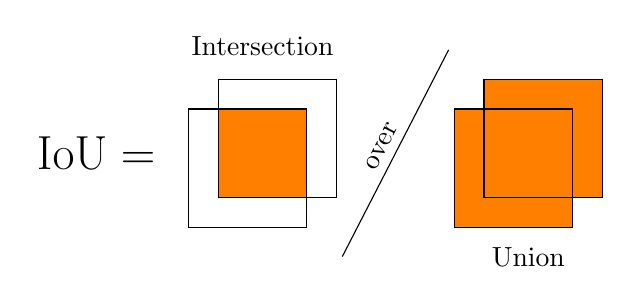
\begin{tikzpicture}[scale=0.75]
  \node[left] at (-0.4, 1.25) {\LARGE $\mathrm{IoU} = $};
  % Intersection illustration
  \begin{scope}
    \clip (0, 0) rectangle (2, 2);
    \fill[orange] (0.5, 0.5) rectangle (2.5, 2.5);
  \end{scope}
  \draw (0, 0) rectangle (2, 2);
  \draw (0.5, 0.5) rectangle (2.5, 2.5);
  \node[above, yshift=0.5em] at (1.25, 2.5) {Intersection};

  % Division sign
  \draw (2.6, -0.5) -- node[auto, sloped] {over} (4.4, 3);

  % Union illustration
  \begin{scope}[shift={(4.5, 0)}]
    \draw[fill=orange] (0, 0) rectangle (2, 2);
    \draw[fill=orange] (0.5, 0.5) rectangle (2.5, 2.5);
    \draw (0, 0) rectangle (2, 2);
    \node[below, yshift=-0.4em] at (1.25, 0) {Union};
  \end{scope}
\end{tikzpicture}

  \caption{%
    Visualization of single-class IoU metric.
  }%
  \label{fig:iou-metric}
\end{figure}

An alternative metric is the dice coefficient, also known as the \textit{$F_1$ score}.
The dice coefficient is defined by taking twice the area of the intersection and dividing by the sum of the areas of the two masks:
%
\begin{equation*}
  \mathrm{F_1}
  =
  \frac{%
    2 \cdot |\mathrm{prediction} \cap \mathrm{truth}|
  }{%
    |\mathrm{prediction}| + |\mathrm{truth}|
  }
  =
  \frac{%
    \mathrm{2 \cdot TP}
  }{%
    2 \cdot \mathrm{TP} + \mathrm{FP} + \mathrm{FN}
  }.
\end{equation*}
%
Again we observe that this metric is bounded to the interval $[0, 1]$, with the same interpretation of the endpoints $0$ and $1$ as with the IoU metric.
The visual representation of this metric is given in \cref{fig:dice-coefficient}.

\begin{figure}[H]
  \centering
  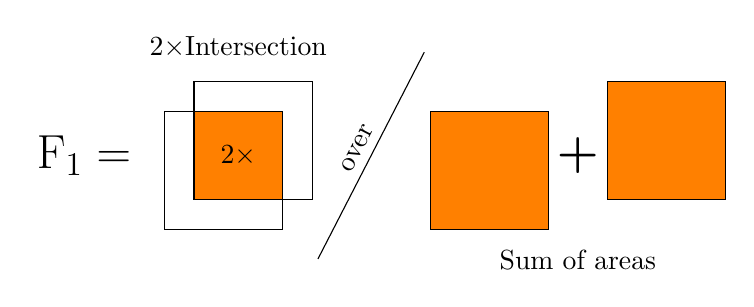
\begin{tikzpicture}[scale=0.75]
  \node[left] at (-0.4, 1.25) {\LARGE $\mathrm{F_1} = $};

  % Intersection illustration
  \begin{scope}
    \clip (0, 0) rectangle (2, 2);
    \fill[orange] (0.5, 0.5) rectangle (2.5, 2.5);
  \end{scope}
  \draw (0, 0) rectangle (2, 2);
  \draw (0.5, 0.5) rectangle (2.5, 2.5);
  \node[above, yshift=0.5em] at (1.25, 2.5) {$2 \times $Intersection};
  \node at (1.25, 1.25) {$2 \times$};

  % Division sign
  \draw (2.6, -0.5) -- node[auto, sloped] {over} (4.4, 3);

  % Union illustration
  \begin{scope}[shift={(4.5, 0)}]
    \draw[fill=orange] (0, 0) rectangle (2, 2);
    \begin{scope}[shift={(2.5, 0)}]
      \draw[fill=orange] (0.5, 0.5) rectangle (2.5, 2.5);
    \end{scope}
    \draw (0, 0) rectangle (2, 2);
    \node[below, yshift=-0.4em] at (2.5, 0) {Sum of areas};
    \node at (2.5, 1.25) {\LARGE \textbf{+}};
  \end{scope}
\end{tikzpicture}

  \caption{%
    Visualization of the single-class dice coefficient metric, also known as the $F_1$ score.
  }%
  \label{fig:dice-coefficient}
\end{figure}

You may have noticed that these two metrics are quite similar; they involve the same quantities, only weighted differently, and map into the same interval.
In fact, we can construct an exact relationship between these two metrics\footnote{The following relationship and the ensuing inequality bounds were noted by the \textit{Cross Validated Stack Exchange} user \enquote{Willem} here: \url{https://stats.stackexchange.com/a/276144}.}
%
\begin{equation*}
  \frac{%
    \mathrm{IoU}
  }{%
    \mathrm{F_1}
  }
  =
  \frac{1}{2}
  +
  \frac{%
    \mathrm{IoU}
  }{%
    2
  }.
\end{equation*}
%
By inspection the two metrics must always be positively correlated, that is, as one metric increases or decreases, the other must follow suit.
A useful insight for understanding how these two metrics actually differ is to observe how the IoU metric is bounded by the dice coefficient:
%
\begin{equation*}
    \frac{%
      \mathrm{F_1}
    }{%
      2
    }
  \leq
    \mathrm{IoU}
  \leq
    \mathrm{F_1}.
\end{equation*}
%
The IoU is \textit{always} less than or equal to the dice coefficient, but never smaller than half the value.
The fraction $\mathrm{IoU} / \mathrm{F_1}$ is equal to 1 whenever the prediction coincides with the ground truth and is equal to $1/2$ whenever there is no overlap at all.
By drawing an analogy to the $p = 1$ (absolute/Manhattan) norm and $p = 2$ (Euclidean) norm, we can say that the $\mathrm{IoU}$ metric weighs the worst case of a prediction more than the average case, and vice versa for the $\mathrm{F_1}$ metric.

\subsection{Binary cross-entropy and soft losses}
So far we have only discussed metrics which are discrete, non-differentiable functions, thus making them unsuitable for direct optimization.
As discussed earlier, we need to introduce a differentiable surrogate loss function which can be optimized.
The key \enquote{trick} is to define a loss function over the continuous probability domain before it is discretized to the classification domain by thresholding.
In order to formulate proper loss functions, we will start by establishing some notation.
Denote the ground truth binary classification mask as $Y \in \mathbb{B}^{H \times W}$ and the corresponding features as $X \in \mathbb{R}^{H \times W \times C}$.
Assume a model $\hat{f}$ parametrized according to $\vec{\theta}$ which provides a probability estimate for $Y$, the probability estimate denoted as $P = \hat{f}(X; \vec{\theta}) \in [0, 1]^{H \times W}$.
For notational convenience we will use a linear index in order to denote single matrix elements, for instance $P_i \in [0, 1]$ for $i = 1, \ldots, HW$.

The most common loss function for binary classification tasks is the \textit{binary cross entropy} (BCE) loss function defined as
%
\begin{equation}
  \mathcal{L}_{\mathrm{BCE}}(P; Y)
  =
  - \sum\limits_{i = 1}^{HW}
  Y_i \log{(P_i)}
  +
  (1 - Y_i) \log{(1 - P_i)}.
  \label{eq:binary-cross-entropy}
\end{equation}
%
However, there are several issues with using the BCE as the loss function for segmentation tasks.
Firstly, it does not take class imbalances into account.
The \textit{weighted binary cross entropy} (wBCE) is one attempt at accounting for class imbalances, but weighting is highly task-dependent and has been shown to have negligible performance improvement over BCE~\cite[p.~98]{soft-losses}.
Another issue with BCE and wBCE is that they are poor surrogates for the segmentation metrics introduced in the previous subsection.
The solution is to introduce differentiable approximations of these discrete segmentation metrics.
Such an approximation for the IoU metric is the \textit{soft Jaccard loss} also known as the \textit{Jaccard distance}~\cite{jaccard-loss-with-equation}, defined by
%
\begin{equation}
  \mathcal{L}_{\mathrm{SJL}}(P; Y)
  =
  1
  -
  \frac{%
    \sum\limits_{i = 1}^{HW}
    P_i Y_i
  }{%
    \sum\limits_{i = 1}^{HW} \left(
      P_i
      +
      Y_i
      -
      P_i Y_i
    \right)
  }
  \approx
  1 - \mathrm{IoU}
  \label{eq:soft-jaccard-loss}
\end{equation}
%
Notice that if $P_i$ is restricted to only take values in $\{0, 1\}$ then $\mathcal{L}_{\mathrm{SJL}}$ becomes equal to $1 - \mathrm{IoU}$.
Other variants exists, and it is also common to add a smoothing factor by adding a value $\delta$ to both the numerator and denominator and multiplying the entire loss with the same value.
A similar differentiable approximation of the dice coefficient, called \textit{soft dice loss}, has also been derived~\cite{original-soft-dice-loss}.

\begin{equation}
  \mathcal{L}_{\mathrm{SDL}}(P; Y)
  =
  \frac{%
    2 \sum\limits_{i = 1}^{HW}
    P_i Y_i
  }{%
    \sum\limits_{i = 1}^{HW} P_i^2
    +
    \sum\limits_{i = 1}^{HW}  Y_i^2
  }
  \approx
  1 - F_1
  \label{eq:soft-dice-loss}
\end{equation}


Optimizing these two metric-sensitive losses have been shown theoretically and empirically to indirectly maximize their respective surrogate metrics~\cite{soft-losses}.
You would think that if the dice coefficient has been chosen as the metric of interest for a given problem, the soft dice loss should be used instead of soft Jaccard loss.
However, \citeauthor{soft-losses} have shown~\cite{soft-losses} that these two metric-sensitive losses are equally good surrogates for each others metrics, and the choice is therefore mainly a preferential one.

\subsection{State-of-the-art}%
\label{sec:segmentation-state-of-the-art}
At the time of this writing, CNNs have largely surpassed all previous methods for performing image segmentation~\cite{segmentation-overview}, but it is still a relatively new field with constantly new improvements being made.
In the following section we will provide an overview of the current state-of-the-art methods being applied within this field, focusing on the unique aspects of each approach.
Four CNN architectures are considered especially influential as they have become essential building blocks for many segmentation architectures; \textit{AlexNet}, \textit{VGG-16}, \textit{GoogLeNet}, and \textit{ResNet}~\cite{segmentation-overview}.
Note that these architectures were initially intended for \textit{classification} and \textit{localization} tasks only, but their conceptual ideas are important for \textit{segmentation} architectures as well.

\textbf{AlexNet}~\cite{segmentation-alexnet} won several image classification competitions when it was first published in~\citeyear{segmentation-alexnet}, including the ILSVRC-2012 competition~\cite{segmentation-overview}.
By employing five convolutional layers, max-pooling layers, ReLU activation functions, and dropout, followed up by a fully connected feedforward classification network, it outperformed the 2nd place contender by a relatively large margin.

The \textbf{VGG-16} architecture~\cite{vgg-16} published in \citeyear{vgg-16} introduced the idea of stacking several convolution filters with small receptive fields in early layers.
VGG-16 distinguishes itself by stacking several convolutional layers with small receptive fields in the first layers instead of using few convolutional layers with large receptive fields.
The result is a network with fewer parameters and more applications of the non-linear activation functions leading to an increased ability to discriminate inputs and reduced training times.
VGG-16 achieved an impressive 92.7\% TOP-5 test accuracy in the ILSVRC-2013 classification competition, inspiring further research involving the techniques employed by the architecture~\cite{segmentation-overview}.

Substantially deep networks are prone to overfitting and are subject to additional computational overhead.
The \textbf{GoogLeNet} architecture~\cite{googlenet} from \citeyear{googlenet} introduced the \textit{inception module} in order to combat this problem, a building block which allow networks to grow in depth and width with modest increases in computational overhead.
The inception module discards the usual approach of ordering convolutions in a sequential manner, instead opting for several parallel pooled convolution branches with different dimensional properties.
Finally a $1 \times 1$ convolution is applied to each branch in order to reduce the dimensionality of the output and the concatenated result is passed onto the next layer.

The \textbf{ResNet} architecture~\cite{resnet} from \citeyear{resnet} was the result of a continued effort to make deeper architectures feasible.
By training a model with 152 layers ResNet won the ILSVRC-2016 competition with a remarkable 96.4\% accuracy~\cite{segmentation-overview}.
This depth is achieved by introducing \textit{skip connections} between layers, an effective way to combat \textit{vanishing gradients}.

The success of convolutional architectures for classification tasks were eventually adapted for segmentation tasks as well.
A fully convolutional, pixel-to-pixel classification network was first published by \citeauthor{segmentation-fcnn} in \citeyear{segmentation-fcnn}~\cite{segmentation-fcnn}.
AlexNet, VGG-16, and GoogLeNet were successfully adapted in order to achieve state-of-the-art performance on the PASCAL-VOC segmentation dataset.

\textit{Fully convolutional neural networks} (FCNN) quickly became the dominant technique used in segmentation challenges after the success in classification and localization challenges.
The \textbf{U-Net} architecture, originally published in \citeyear{segmentation-unet} and intended for biomedical image segmentation, has become one of the more popular segmentation architectures.
U-Net has an \textit{encoder/decoder}-structure; the network starts with a contracting path where context is extracted from the input image.
This is followed by a symmetric expanding path in order to upscale the segmentation to the original resolution by the use of \textit{transposed convolution}, a trainable procedure also known as \textit{deconvolution}.
\textit{Skip-connections} are introduced in order to forward information from the contracting layers to the respective expanding layers.
\textbf{SegNet}~\cite{segmentation-segnet}, an architecture from the same time period, has a similar encoder/decoder structure as U-Net.
The difference between the two architectures is that SegNet only copies over the max-pool indices in the skip connections instead of forwarding the entire feature layer, thus decreasing the memory requirements of the network.

\textbf{R-CNN}~\cite{r-cnn}, and the subsequent improvements \textbf{Fast R-CNN}~\cite{fast-r-cnn} and \textbf{Faster R-CNN}~\cite{faster-r-cnn}, made great strides in image classification and localization tasks in \citeyear{r-cnn} and \citeyear{faster-r-cnn}.
The crux of their success lies in the \textit{region proposal network} (RPN), a parallel network which is responsible for identifying \textit{regions of interest} (RoIs) in the convolved feature maps.
These RoIs are transformed to consistent dimensions by a custom pooling method called \textit{RoIPool}, or alternatively \textit{RoIWarp}, and subsequently classified and localized with a fully connected feedforward network.
\textbf{Mask R-CNN}~\cite{mask-r-cnn}, published by the Facebook AI research group in \citeyear{mask-r-cnn}, sought to expand Faster R-CNN in order to predict segmentation as well.
Mask R-CNN replaces RoIPool with \textit{RoIAlign}, a region of interest pooling method which preserves a one-to-one pixel mapping between the original feature map and the extracted region of interest.
The output of the pooling operation is forwarded to a parallel FCNN branch in order to perform pixel-wise segmentation.
This segmentation branch predicts independent masks without inter-class competition, and reuses the work performed by the classification branch in order to select which mask to apply to a given region.

\textbf{Capsule networks} has become a topic of large interest in the research community as of late.
First introduced in a paper~\cite{capsules} by \citeauthor{capsules}, it has since been applied to segmentation tasks as well.
One such adaption is the \textbf{SegCaps} architecture~\cite{segmentation-segcaps}.
The main idea behind capsule networks is to output more data from each neuron, effectively allowing the network to make more informed decisions with this new context.
Instead of only storing a single scalar in each neuron they store a contextual vector instead.
Each vector encodes information about the spatial orientation, magnitude, prevalence, and other attributes related to the extracted features.
These \textit{capsule vectors} are \textit{dynamically routed} to the capsules in the next layer based on vector similarity.

\subsection{The U-Net model architecture}%
\label{sec:unet}
We have chosen the U-Net architecture for segmenting building outlines and we will present numerical experiments in \cref{sec:experiments}.
The U-Net model has already been briefly described in the previous section and the architecture has been illustrated in \cref{fig:unet}, but we will provide a more detailed summary of the U-Net architecture here.
An alternative visual representation of the U-Net architecture is provided in \cref{fig:unet2}.

\begin{figure}[H]
  \centering
  \includegraphics[width=0.75\textwidth]{Unet_ushape}
  \caption{%
    U-Net model architecture.
    The vertical axis denotes the resolution of the features, resulting in the U-shape of U-Net.
    Figure has been generated by modifying a \texttt{tikz} example provided in the MIT licenced \texttt{PlotNeuralNet} library available at this URL:\@
    \protect\url{https://github.com/HarisIqbal88/PlotNeuralNet}.
  }%
  \label{fig:unet2}
\end{figure}

As can be seen in \cref{fig:unet2}, the U-Net architecture consists of four sequential \enquote{encoder modules}, each module applying a set number of convolutional filters followed by the application of the ReLU activation function.
The number of trained convolutional filters in each encoder module is respectively: 64, 128, 256, and 512.
Each module ends with a downsampling operation in form of max-pooling of size 2.
Since our input images have resolution $256 \times 256$, we end up with inputs of size $16 \times 16$ to the \enquote{bottleneck convolution module} where 1024 convolutional filters are trained.
The bottleneck convolution module is placed at the bottom of the U-shape in \cref{fig:unet2}.
Each decoder block utilizes batch normalization and max-pooling dropout, although models without these building blocks will be tested in \cref{sec:technique-experiments}.
The \enquote{decoder modules} apply transposed convolutions in order to upsample the resolution by a factor of two, the number of filters being equivalent to their respective \enquote{mirror encoders}, i.e.\ the encoder modules handling inputs with identical resolutions.
Four such modules are applied in order to yield a final output resolution of size $256 \times 256$, the original input resolution.
The outputs of the mirror encoder modules are concatenated to the input to the decoder modules in order to aid the upsampling procedure.
Finally, a sigmoid convolution with filter size \num{1} is applied in order to produce the final segmentation probabilities.
This model has been implemented using the declarative Keras API in Tensorflow v2.0 and the source code is available at the \texttt{JakobGM/project-thesis}\todo{Add relevant code in appendix instead.} repository on GitHub%
\footnote{%
  All source code used in order to produce and present the results in this paper are available from the following public GitHub repository: \url{https://github.com/JakobGM/project-thesis}.
  Specifically, the implementation of the U-Net architecture has been made available here: \url{https://github.com/JakobGM/project-thesis/blob/master/remsen/models.py}.
}.
The final network has \num{7025329} trainable parameters.


\section{Surface Raster Model}
\subsection{State-of-the-art}
\subsection{A modified U-Net architecture for surface normal raster prediction}
\subsection{Normal losses}

\section{Optimization}
\subsection{Multitask learning}


\section{Raster Normalization}%
\label{sec:raster-normalization}
Input data normalization has been found to be of vital importance when training neural networks, in certain cases reducing predictive errors by several orders of magnitude and training times by one order of magnitude~\cite{input_normalization_1997}.
How to normalize input data depends on distribution of the feature space, which will be investigated here.

\subsection{RGB rasters}

A given RGB pixel is an unsigned 8-bit integer and therefore takes values in a bounded, integer domain
%
\begin{equation*}
  I_{i,j,c} \in \{0, 1, \ldots, 255\}, \text{ for } c \in \{r, g, b\}.
\end{equation*}
%
The distribution of each color channel over the entire coverage area of the Trondheim aerial photography data set is shown in \cref{fig:rgb-density}, and aggregate statistics for each channel are listed in \cref{tab:rgb-statistics}.

\begin{figure}[H]
  \begin{floatrow}
    \ffigbox[8.5cm]{%
      \includegraphics[width=\linewidth]{rgb-density}
    }{%
      \caption{%
        Distribution density for all three color channels in the aerial photography data set covering Trondheim municipality (2017).%
        \label{fig:rgb-density}
        %Peak at 64 and 191.
      }%
    }
    \hspace{-2.5em}
    \inlinetable{%
      \scalebox{0.85}{%
        \begin{tabular}{%
          l
          S[round-mode=places, round-precision=1]
          S[round-mode=places, round-precision=1]
        }
          \toprule
          {Channel} & {Mean [1]} & {SD [1]} \\
          \midrule
          \textcolor{red}{Red} & 101.60925940814 & 55.010463592563 \\
          \textcolor{green}{Green} & 102.67104002891 & 48.740409963323 \\
          \textcolor{blue}{Blue} & 91.286001382234 & 37.216349915699 \\
          \bottomrule
        \end{tabular}
      }
      \vspace{5em}
    }{%
      \caption{%
        Aggregate statistics for each image channel distribution for the aerial photography data set covering Trondheim municipality (2017).%
        \label{tab:rgb-statistics}
      }%
    }
  \end{floatrow}
\end{figure}

The image channels can be easily normalized to the domain $[0, 1]$ by dividing by $255$ across all three image channels.
This is in essence a lossless transformation, since the normalization function $f(x) = x/255$ is trivially invertible, and thus no information is lost by this normalization.

\subsection{LiDAR rasters}

The \enquote{$z$ channel} represents elevation data from the respective digital surface model.
Elevation measurements are represented by 32-bit, single-precision floating point numbers, and can theoretically take values in the domain $I_{i,j,z} \in (\SI{-3.4e38}{\meter},\allowbreak\SI{3.4e8}{\meter})$.
In practice, the measurements are bounded by the regional extrema, $(\SI{-433}{\meter},~\SI{8848}{\meter})$ for dry land globally, and $(\SI{-9}{\meter},~\SI{569}{\meter})$ for the Trondheim region.
The distribution of $z$ channel values for the Trondheim region is shown in \cref{fig:elevation-density}, and aggregate statistics are listed in \cref{tab:elevation-statistics}.

\begin{figure}[H]
  \begin{floatrow}
    \ffigbox[8cm]{%
      \includegraphics[width=\linewidth]{elevation-density}
    }{%
      \appcaption{%
        Distribution density for elevation data set covering Trondheim municipality (2017).
      }{%
        Outlier values $(\SI{0}{\meter}, \SI{2.74}{\percent})$ and $(\SI{148}{\meter}, \SI{1.93}{\percent})$ have been cropped.
      }%
      \label{fig:elevation-density}
    }
    \hspace{-1.8em}
    \inlinetable{%
      \scalebox{0.70}{%
        \begin{tabular}{%
          l
          S[round-mode=places, round-precision=1]
          S[round-mode=places, round-precision=1]
        }
          \toprule
          {Channel} & {Mean [m]} & {SD [m]} \\
          \midrule
          Elevation & 155.36339532445 & 116.52777315076 \\
          \bottomrule
        \end{tabular}
      }
      \vspace{7em}
    }{%
      \caption{%
        Aggregate statistics for elevation data set covering municipality of Trondheim (2017).
      }%
      \label{tab:elevation-statistics}
    }
  \end{floatrow}
\end{figure}

A normalization technique analogue to the RGB min-max scaling for elevation tile number $k$, denoted as $Z^{(k)}$, would therefore be
\begin{align*}
  \hat{Z}_{i,j}^{(k)}
  &=
  \frac{%
    Z_{i,j}^{(k)} - \underset{t \in \mathrm{TRD}}{\min}~Z^{(t)}
  }{%
    \underset{t \in \mathrm{TRD}}{\max}~Z^{(t)} - \underset{t \in \mathrm{TRD}}{\min}~Z^{(t)}
  }
  \tag{Global min-max normalization}
  \\
  &=
  \frac{%
    Z_{i,j}^{(k)} + \SI{9}{\meter}
  }{%
    \SI{578}{\meter}
  },%
\end{align*}

where $\mathrm{TRD}$ is the index set of all tiles belonging to the Trondheim region.
The normalized raster elevation values in $\hat{Z}^{(k)}$ are guaranteed to be bounded to the interval $[0, 1]$, as with the RGB raster.
In order to evaluate if this will properly normalize the $z$ raster channel across tiles, we plot the \enquote{tile-by-tile} $z$ channel statistics in \cref{fig:elevation-spread}.

\begin{figure}[H]
  \centering
  \includegraphics[width=\linewidth]{elevation-spread}
  \appcaption{%
    Elevation value statistics for a tile subset of sample size $n = \num{10000}$.
  }{%
    The left figure shows the minimum, mean, and maximum elevation, sorted by increasing mean from left to right.
    The right figure shows the histogram of the tile elevation \textit{ranges} (difference between maximum elevation and minimum elevation within tile).
  }%
  \label{fig:elevation-spread}
\end{figure}

While the global elevation range is $\SI{569}{\meter} - (\SI{-9}{\meter}) = \SI{578}{\meter}$, the elevation range within each respective tile is on average approximately $\SI{22}{\meter} \pm \SI{8}{\meter} (\mathrm{SD})$, that is, much less than \SI{578}{\meter}.
Coupled with the fact that the tile elevation \textit{means} are somewhat uniformly distributed between \SI{0}{\meter} and \SI{200}{\meter}, ignoring the right tail, a global normalization will yield tile elevation values with small standard deviations and highly variable means.
We can therefore conclude that global min-max scaling is not suitable for the elevation image channel.
A proposed solution to this problem is to scale each tile independently to the domain $[0, 1]$, what we will refer to as \enquote{local min-max normalization}.
%
\begin{align*}
  \hat{Z}_{i,j}^{(k)}
  &=
  \frac{%
    Z_{i,j}^{(k)} - \min~Z^{(k)}
  }{%
    \max~Z^{(k)} - \min~Z^{(k)}
  }%
  \tag{Local min-max normalization} % chktex 35
  \\
  &=
  \frac{%
    Z_{i,j}^{(k)} - \beta
  }{%
    \alpha - \beta
  },%
  &\text{where }\alpha \defeq \max~Z^{(k)},~\beta \defeq \min~Z^{(k)}.
\end{align*}

The scaling factor $\alpha - \beta$ is constructed such that the normalized tile minimum becomes 0 and maximum becomes 1 for all tiles.

Any elevation normalization method must account for the fact that missing data values are replaced by a pre-defined \texttt{nodata} placeholder value, usually \SI{-3.4e38}{\meter}.
Otherwise a large negative bias is introduced for all tiles with any missing data.
Leaving \texttt{nodata} values unnormalized with such extreme values will heavily influence the weighted sum calculated by nodes in any neural network, and must therefore filled in with values from the normalized domain.
Filling in $0$ values for all \texttt{nodata} indices has been shown to work well in most cases.
The \enquote{\texttt{nodata}-aware} min-max normalization algorithm used for preprocessing elevation input data is given in \cref{alg:local-min-max-scaling}.

\begin{algorithm}{Nodata-aware local min-max normalization}{alg:local-min-max-scaling}
  \item Calculate the valid index set defined by $\mathcal{V} = \{(i, j): Z_{i,j} \neq \texttt{nodata}\}$.
  \item Calculate $\alpha = \underset{(i,j) \in \mathcal{V}}{\max} Z_{i,j}$ and $\beta = \underset{(i,j) \in \mathcal{V}}{\min} Z_{i,j}$.
  \item Construct normalized raster defined by
    \begin{equation*}
        \hat{Z}_{i,j} = \begin{cases}
          \frac{Z_{i,j} - \beta}{\alpha - \beta}, & \text{if } (i,j) \in \mathcal{V}, \\
          0, & \text{otherwise.}
        \end{cases}
    \end{equation*}
\end{algorithm}

One of the core issues with local min-max normalization is that it is essentially a lossy operation.
As each tile is independently scaled, it is no way to accurately reconstruct the original elevation map in metric units.
One way to determine if a roof-like surface belongs to a proper building or a shed, for instance, is to inspect its relative height, which becomes impossible without knowing the relative scaling of each tile with respect to each other.
We therefore hypothesize that the variable scaling imposed by local min-max normalization could impede the performance of models trained on such data.
An alternative normalization method is therefore proposed where the scaling factor $\alpha - \beta$ is replaced by a predefined \textit{constant} scaler $\gamma > 0$.
The translation $\beta$ is kept as-is since there is no reason to distinguish between cadastral plots situated at sea-level and other altitudes when it comes to building outline detection.
This \enquote{metric normalization} is therefore defined as:

\begin{equation*}
  \hat{Z}_{i,j}^{(k)}
  =
  f\left(Z_{i,j}^{(k)}\right)
  =
  \frac{%
    Z_{i,j}^{(k)} - \min~Z^{(k)}
  }{%
    \gamma
  },%
  \hspace{2em} \gamma > 0.
  \tag{Metric normalization} % chktex 35
  \label{test}
\end{equation*}

Elevation values in the $z$ channel now have a consistent physical interpretation given in units $\si{\meter} / \gamma$ across all tiles.
The modified metric normalization method is provided in \cref{alg:metric-normalization}.

\begin{algorithm}{Nodata-aware metric normalization}{alg:metric-normalization}
  \item Calculate the valid index set defined by $\mathcal{V} = \{(i, j): Z_{i,j} \neq \texttt{nodata}\}$.
  \item Calculate $\beta = \underset{(i,j) \in \mathcal{V}}{\min} Z_{i,j}$ and define a global scaler $\gamma > 0$.
  \item Construct normalized raster defined by
    \begin{equation*}
        \hat{Z}_{i,j,z} = \begin{cases}
          \frac{Z_{i,j} - \beta}{\gamma}, & \text{if } (i,j) \in \mathcal{V}, \\
          0, & \text{otherwise.}
        \end{cases}
    \end{equation*}
\end{algorithm}

A comparison of these two normalization methods, \cref{alg:local-min-max-scaling} and \cref{alg:metric-normalization} that is, will be provided in \cref{sec:normalization-experiment}.\todo{Will this still be true?}



\chapter{Post-processing}%
\label{chap:post-processing}

Assume that we have two machine learning models; firstly $\segmodel$ which is able to predict \emph{semantic} segmentation masks $\predsegraster$, and secondly $\normmodel$ which is able to predict surface normal rasters $\prednormraster$.
These two models could conceivably be sub-models of a \emph{single} multi-task model, both accepting remote sensing data in the form of aerial photography and/or LiDAR measurements as illustrated in \cref{fig:multitask-prediction}.
\begin{figure}[H]
  \centering
  \includegraphics{multitask-prediction.tikz}
  \caption{%
    Demonstration of unprocessed output from a surface raster machine learning pipeline.
  }%
  \label{fig:multitask-prediction}
\end{figure}
\noindent
As discussed in \cref{sec:surface-rasterization} -- \enquote{\nameref{sec:surface-rasterization}}, the goal is to convert these two model predictions belonging to the surface \emph{raster} domain $R$ back to the \emph{vector} polygon domain $V$ by constructing a suitable pseudoinverse mapping $m^{\dagger}: R \rightarrow V$ as illustrated in \cref{fig:pseudoinverse}.
\begin{figure}[H]
  \centering
  \includegraphics{pseudoinverse.tikz}
  \caption{Pseudoinverse mapping, $m^{\dagger}$, mapping from the raster domain to the vector domain.}%
  \label{fig:pseudoinverse}
\end{figure}
\noindent
More specifically, we will construct a pseudoinverse mapping which accepts two inputs, a predicted surface normal raster and a semantic segmentation map, and produces three-dimensional vector polygons, which we will denote as $\predpolygons$,
\begin{equation*}
  \predpolygons
  \defeq
  \pseudoinverse\left(
    \predsegraster,
    \prednormraster
  \right).
\end{equation*}
This pseudoinverse mapping should produce three-dimensional polygons which can be considered close to the ground truth polygons $\polygons$, where the notion of \enquote{closeness} between $\predpolygons$ and $\polygons$ is expressed in a \textit{polygon distance metric} $d: V \times V \rightarrow \mathbb{R}$.
The main objective of the pseudoinverse mapping is therefore to minimize
\begin{equation*}
  d\left(
    \predpolygons,
    \polygons
  \right)
  =
  d\left(
    \pseudoinverse\left(\predsegraster, \prednormraster\right),
    \polygons
  \right).
\end{equation*}
The model predictions, $\predsegraster$ and $\prednormraster$, are not perfect, and the pseudoinverse should therefore be \textit{robust} relative to the types of errors commonly produced by the models, $\segmodel$ and $\normmodel$, producing minimal error as defined by the distance metric $d$.
Constructing a suitable pseudoinverse is therefore not only highly dependent on the surface raster format itself, but also the specific behaviour of the models used to produce the raster format.
In the evaluation of a pseudoinverse mapping it may still be beneficial to take the models themselves out of the equation by replacing the predicted rasters with the ground truth rasters $m(\polygons)$, thus verifying that the pseudoinverse mapping also minimizes
\begin{equation*}
  d\left(
    \pseudoinverse\left(m\left(\polygons\right)\right),
    \polygons
  \right).
\end{equation*}
A pseudoinverse mapping which performs badly under this \enquote{round-trip metric} will likely perform badly under the pseudoinverse mapping of model predictions as well.
\newpage

In the following sections we will present a pseudoinverse mapping which is considered highly suitable for producing roof surface polygons, a mapping which encodes our specific domain knowledge about the general geometric properties of roof surfaces.
Our main idea is to use the predicted surface normal raster in order to \textit{partition} the \textit{semantic} segmentation map into an \textit{instance} segmentation map, where the instance segmentation map can subsequently be used in order to construct enclosing vector polygons for each instance.
The three-dimensional orientation of each polygon can finally be inferred from the predicted surface normals in conjunction with the original LiDAR data.

Our implementation applies a divide-and-conquer approach to the problem by dividing the semantic segmentation map into mutually disjunct sub-regions and partitioning these sub-regions entirely independent of each other.
This first-pass partitioning is described in \cref{sec:connected-region-labeling} -- \enquote{\nameref{sec:connected-region-labeling}}.
A second-pass partitioning is performed by grouping together connected regions which share the same normal vector orientation.
The task of determining which pixels $(i, j)$ which share the same values for $N_{i, j}$ is formulated as a \textit{clustering problem}, the solution of which will be presented in \cref{sec:instance-clustering}.
A final conversion of instance segmentation maps to vector polygons will be described in \cref{sec:vectorization}.

Before delving into the details of the implementation, we begin by summarizing the entire post-processing algorithm in conceptual terms:

\begin{leftbar}
  \noindent
  Given a predicted segmentation map $\predsegraster$ and surface normal raster $\prednormraster$:
  \begin{itemize}[leftmargin=*]
    \item Threshold segmentation activations $\predsegraster$ according to some tolerance $\texttt{TOL}$ in order to construct \emph{binary} segmentation raster $\predbinarysegraster$.
    \item Identify connected sub-regions of the binary segmentation raster $\predbinarysegraster$, and sub-divide the following processing independently across these sub-regions.
    \item Apply a conservative clustering algorithm which does \emph{not} require the specification of the number of clusters \textit{a priori}.
    \item Apply a second clustering algorithm which encodes suitable domain knowledge in order to classify the remaining points, producing a labeled partition of the original binary segmentation raster.
    \item Construct two-dimensional vector polygons which enclose each instance region.
    \item Simplify these vector polygons.
    \item Reconstruct $z$-coordinates of each polygon vertex.
  \end{itemize}
\end{leftbar}


\newpage
\section{Connected region labeling}%
\label{sec:connected-region-labeling}
The predicted segmentation map $\predsegraster$ produced by $\segmodel$ is a $H \times W \times 1$ raster array with values in the continuous domain $[0, 1]$, values $\predsegraster_{i,j}$ which can be interpreted as the model's confidence in there being a roof surface at pixel location $(i, j)$.
In order to make an actual binary prediction, we \textit{threshold} the segmentation map, creating a binary segmentation map $\predbinarysegraster$ defined by
\begin{equation*}
  \predbinarysegraster \defeq \predsegraster > \texttt{TOL}
  \iff
  \predbinarysegraster_{i, j}
  =
  \begin{cases}
    1, &\text{if } \predsegraster_{i, j} > \texttt{TOL}. \\
    0, &\text{otherwise.}
  \end{cases}
\end{equation*}
We will use the most commonly used threshold value, naturally $\texttt{TOL} = 0.5$.
The process of thresholding has been illustrated in \cref{fig:activation-thresholding}.
\begin{figure}[H]
  \centering
  \includegraphics{activation-thresholding.tikz}
  \caption{Thresholding model segmentation prediction in order to create a \textit{binary} segmentation map.}%
  \label{fig:activation-thresholding}
\end{figure}
\noindent
This binary segmentation map can now be used in order to segment the predicted surface normal raster as well, producing what we will refer to as a \textit{segmented surface normals}.
The segmented surface normal raster can be easily produced by taking the element-wise product of the predicted surface normal raster and the thresholded binary segmentation map, which we will denote as $\predbinarysegraster \odot \prednormraster$, and is formally defined as
\begin{equation*}
  \predsegnormraster \defeq \predbinarysegraster \odot \prednormraster
  \iff
  \predsegnormraster_{i, j}
  =
    \predbinarysegraster_{i, j}
    \cdot
    \left[\prednormraster_{i,j,x}, \prednormraster_{i,j,y}, \prednormraster_{i,j,z}\right].
\end{equation*}
The effect of segmenting the predicted surface normal raster is illustrated in \cref{fig:normal-segmentation}.
\begin{figure}[H]
  \centering
  \includegraphics{normal-segmentation.tikz}
  \caption{Demonstration of segmenting a predicted surface normal raster using a thresholded segmentation map.}%
  \label{fig:normal-segmentation}
\end{figure}
\noindent
We have now found an index set, $\mathcal{I}$, for which there is predicted to contain a polygon.
\begin{equation*}
  \mathcal{I}
  =
  \left\{
  (i, j)
  ~\big{|}~
  \left|\predpolygons\left(\pixtogeo{i}{j}\right)\right| > 0
  \right\}
\end{equation*}
We now need to assign a single label to each such coordinate, indicating which polygon $P \in \predpolygons$ the given coordinate belongs to.
We apply a divide-and-conquer approach by partitioning the thresholded segmentation map into those regions which are connected.
This can be performed by a so-called \textit{connected region labeling} algorithm, and has been illustrated in \cref{fig:mask-iteration}.
\begin{figure}[H]
  \centering
  \includegraphics{mask-iteration.tikz}
  \caption{The result of the  \textit{connected region labeling} algorithm applied on the thresholded segmentation map.}%
  \label{fig:mask-iteration}
\end{figure}
\noindent
The example presented in \cref{fig:mask-iteration} shows that there exists four, separate connected regions ($A$, $B$, $C$ and $D$).
If we assume that the segmentation map is correct, then we can conclude that any polygon belonging to one of these regions will not belong to any other region.
We can therefore solve the partition of each region as entirely independent tasks.
The partitioning of each connected sub-region is now formulated as a normal vector clustering problem.


\newpage
\section{Instance Clustering}%
\label{sec:instance-clustering}
\subsection{DBSCAN}

\subsection{\texorpdfstring{$k$}{k}-nearest neighbour noise fitting}


\section{Vectorization}%
\label{sec:vectorization}
\subsection{Two-dimensional polygonization}

\subsection{Three-dimensional fitting}


\section{Simplification}%
\label{sec:simplification}
\subsection{Ramer–Douglas–Peucker algorithm}

\begin{figure}[H]
  \centering
  \includegraphics[]{polygon-simplification.tikz}
  \caption{Polygons before and after RDP has been applied.}
\end{figure}

\begin{figure}
  \centering
  \includegraphics{rdp-algorithm.tikz}
  \appcaption{%
    Illustration of the Ramer-Douglas-Peucker algorithm.
  }{%
    This specific example has been recreated from Figure~5 in~\cite{original-rdp-figure}.
  }
  \label{}
\end{figure}


\begin{figure}
  \centering
  \includegraphics[scale=0.45]{img/tile-data/34-0/surface_normals_3+segmented_normals_2/predicted_segmented_normals}
  \includegraphics[scale=0.45]{img/tile-data/34-0/true_normals}
  \includegraphics[scale=0.45]{img/tile-data/34-0/segmented_normals_2/activations}
  \\
  \includegraphics[scale=0.45]{img/tile-data/34-0/surface_normals_3/predicted_normals}
  \includegraphics[scale=0.45]{img/tile-data/34-0/segmented_normals_2/confusions}
  \includegraphics[scale=0.45]{img/tile-data/34-0/true_mask}
  \\
  \hspace{2.15em}\includegraphics[scale=0.45]{img/tile-data/34-0/surface_normals_3/cosine_similarity}
\end{figure}

\chapter{Experiments}%
\label{sec:experiments}

\section{Experimental Setup}
\subsection{Training procedure}
\subsection{Software}
\subsection{Hardware and performance}

\section{Features}
\subsection{LiDAR data}

\begin{figure}[H]
  \includegraphics[width=0.75\textwidth]{img/training/normals_with_only_lidar-train+validation-loss.pdf}
  \caption{TODO}
\end{figure}

\subsection{RGB data}

\begin{figure}[H]
  \includegraphics[width=0.75\textwidth]{img/training/normals_with_only_rgb-train+validation-loss.pdf}
  \caption{TODO}
\end{figure}

\begin{figure}[H]
  \includegraphics[width=0.75\textwidth]{img/training/normals_with_only_lidar+normals_with_only_rgb-train+validation-loss.pdf}
  \caption{TODO}
\end{figure}

\subsection{LiDAR+RGB data}

\begin{figure}[H]
  \includegraphics[width=0.75\textwidth]{img/training/normals_with_lidar_and_rgb-train+validation-loss.pdf}
  \caption{TODO}
\end{figure}

\begin{figure}[H]
  \includegraphics[width=0.75\textwidth]{img/training/normals_with_lidar_and_rgb+normals_with_only_lidar+normals_with_only_rgb-validation-loss.pdf}
  \caption{TODO}
\end{figure}

\begin{figure}[H]
  \includegraphics[width=0.75\textwidth]{img/training/normals_with_lidar_and_rgb+normals_with_only_lidar+normals_with_only_rgb-train+validation-loss.pdf}
  \caption{TODO}
\end{figure}


\section{Architecture}
\subsection{Multitask learning}\label{sec:multitask-experiments}
\begin{figure}[H]
  \includegraphics[width=\linewidth]{multitask-alpha-train.pdf}
  \caption{Training losses.}
\end{figure}

\begin{figure}[H]
  \includegraphics[width=\linewidth]{multitask-alpha-validation.pdf}
  \caption{Validation losses.}
\end{figure}

\begin{figure}[H]
  \includegraphics[width=\linewidth]{best-alphas.pdf}
  \caption{Best alpha for each split and each loss.}
\end{figure}

\begin{figure}[H]
  \includegraphics[width=\linewidth]{training/multitask-train+validation-loss.pdf}
  \caption{Training of multitask network.}
\end{figure}

\begin{figure}[H]
  \includegraphics[width=\linewidth]{training/multitask+normals_with_lidar_and_rgb-train+validation-surface_normal_loss.pdf}
  \caption{Multitask vs single-task surface normal network (training + validation split).}
\end{figure}

\begin{figure}[H]
  \includegraphics[width=\linewidth]{training/multitask+segmentation_with_lidar_and_rgb-train+validation-surface_segmentation_loss.pdf}
  \caption{Multitask vs single-task surface segmentation network (training + validation split).}
\end{figure}


\chapter*{Conclusion and Further Work}

\begin{itemize}
  \item Other polygon simplification methods.
  \item Visualizing normal vectors preserving distances.
  \item Image augmentation using transformations of normal vectors.
  \item Using different architectures for appending three-output channels.
  \item Using different activation functions in output layer of normal vector.
\end{itemize}


\chapter*{\bibname}
\emergencystretch=2em % Insert line breaks correctly on long URLs and titles in bibliography
\printbibliography[heading=none]

\chapter{Additional Material}
\label{app:additional}

\section{Mapping Between Coordinate Systems}

\section{Zero-Buffering Vector Datasets}

\section{Merging Raster Datasets}

\section{A Note on Visualizing Surface Normals}
\todo{Write about surface normal visualization.}


\section{A Keras Layer Implementation of LiDAR Normalization}


\end{document}
